\documentclass{report}

\usepackage[utf8]{inputenc}
\usepackage[francais]{babel}
\usepackage{url}
\usepackage{color}
\usepackage{listings}
\usepackage{graphicx}


\definecolor{vert}{rgb}{0,0.5,0.1} 
\definecolor{blue}{rgb}{0,0.4,0.6} 
\definecolor{red}{rgb}{1,0,0} 
\definecolor{out}{rgb}{0.6,0.6,0.6} 
\lstset{inputencoding=utf8,
				language=C,
				showstringspaces=false,
				tabsize=2,
				basicstyle=\scriptsize,
				keywordstyle=\color{vert},
				commentstyle=\color{blue}, 
				stringstyle=\color{red}
}
\lstnewenvironment{codeoutput}
	{\lstset{basicstyle=\ttfamily\color{out},
	}}
{}


\title{TER, développement d'un émulateur de \\Game Boy}
\author{BERGER Mickaël \\ DIVET Joachim \\ VINARD Florian}
\date{17 Mai 2013}

\begin{document}
\maketitle
\chapter*{Remerciements}
Nous souhaitons tout d'abord remercier M. William PUECH notre tuteur qui a bien voulu nous encadrer pour ce travail d'études et de recherches, ainsi que son doctorant M. Vincent ITIER qui a été présent lors des réunions. \\Nous remercions également la communauté présente sur internet qui participe activement au développement d'émulateurs ainsi qu'à la rédaction de documentations abordables. Et tout spécialement le dénommé "Blargg" qui a produit et mis à disposition toutes sortes d'outils destinés au développement d'émulateurs.

\tableofcontents
\listoffigures

\chapter*{Introduction}
	Dans le cadre de la 1ère année de Master Informatique à l'Université de Montpellier
	2, tous les élèves de la promotion ont été amenés à réaliser un projet
	sous tutelle, afin de mettre en pratique les compétences acquises
	durant nos précédentes années d'études, mais aussi et surtout de nous
	placer dans un contexte de réel travail sur un projet à réaliser.\\
	Ce Travail d'Étude et de Recherche est donc un bon moyen de nous
	familiariser avec le type de travail qui pourra nous être demandé dans
	les années à venir, ainsi que de travailler nos démarches.
	Et c'est sur l'élaboration d'un Émulateur de console de jeu vidéo, et plus précisément de Game Boy,
	que nous avons choisi de travailler, plus que motivé par l'apport de
	connaissances que représente l'étude du comportement d'un processeur
	et sa simulation à partir de zéro.
	\\
	L'idée principale n'étant pas simplement de pouvoir rejouer aux jeux
	ayant bercé notre enfance, mais bien d'analyser et comprendre le
	fonctionnement d'un système d'émulation, qui reste très orienté bas
	niveau et "culture des composants", mais suffisamment accessible pour
	que notre travail puisse aboutir à un exemple concret, réalisé par nos
	soins.\\
	\\

\section*{Définition du projet}
\subsection*{Qu'est ce qu'un émulateur?}
	Selon la définition d'émulation sur le site Wikipédia:\\"\textbf{En informatique, l'émulation consiste à substituer un élément de matériel informatique – tel un terminal informatique, un ordinateur ou une console de jeux – par un logiciel.}".\\Ce logiciel est donc ce que l'on appelle un émulateur.
\subsection*{Qu'est ce que la Game Boy?}
	La Game Boy est une console de jeu portable commercialisée par Nintendo en Europe durant l'année 1990.
\subsection*{Déroulement}
	Dès lors que notre choix fut fixé et validé par nos enseignants, il
	fut assez rapide de déterminer les grandes lignes du déroulement du
	projet, à savoir une première étape de documentation importante, afin
	de bien comprendre le fonctionnement de l'appareil. Une seconde partie
	de développement et donc de réelle simulation des différents aspects
	du système, et une dernière partie de perfectionnement et
	amélioration éventuelle de ce que nous aurons réalisé.

\chapter{Organisation du projet}
\section{Choix des outils}
Ce projet a été réalisé grâce à de nombreux outils, les voici, avec les raisons qui ont motivés nos choix.\\
Si cette partie est importante, le nombre de projets que nous avons déjà réalisé par le passé nous a apporté une expérience et un bagage suffisants pour prendre ces décisions rapidement. Les motivations présentés ci-dessous sont par conséquent d'apparences courtes, mais la réflexion qui a précédé les choix n'en a pas pour autant été altérée.

\subsection{Environnement de travail}
\textbf{Linux}, car il est confortable pour les développeurs. Linux dispose dans la plupart des distributions classiques d'un ensemble d'outils pour développer tel que gcc, gdb, etc. De plus l'installation de librairies et/ou de logiciels supplémentaires est relativement aisée grâce au système de logithèques.

\subsection{Langage}
\textbf{C}, un des langages les plus utilisés dans le monde de l'émulation. Il permet d'obtenir des exécutables compilés rapides, et selon les compilateurs de mettre en place des stratégies d'optimisations, afin de rendre l'émulateur plus fluide et rapide.

\subsection{Compilateur}
\textbf{gcc}, compilateur du langage C, il accepte beaucoup d'options permettant d'optimiser l'exécutable compilé.

\subsection{Librairie multimédia}
\textbf{SDL}, une librairie multimédia pour le langage C. Elle dispose d'un ensemble de primitives permettant de gérer tout ce qui est nécessaire pour créer un jeu en 2D et donc un émulateur de Game Boy: affichage de fenêtre, son, interruptions et autres.

\subsection{Dépôt}
\textbf{Github}, un site permettant de créer gratuitement un dépôt git. git est un logiciel de contrôle de version, permettant aux membres d'un même projet de modifier ce projet, en faisant en sorte que chacun puisse travailler sur la même version. Le lien vers notre dépôt se trouve sur la page de bibliographie à \cite{github}.

\subsection{IDE}
Le projet n'a pas été conçu avec un IDE particulier. Lors de la conception du projet il a été propre à chacun d'utiliser l'IDE qui lui convient. Cependant la plupart du code a été édité avec l'éditeur de texte \textbf{Vim}.

\subsection{Documentation et Information}
Comme indiqué un peu plus haut, l'étude de la documentation a occupé une part importante de notre projet. Nous avons donc du nous concerter pour se mettre d'accord sur les documentations à utiliser, étant donné leur nombre, afin de ne pas être victime des petites différences que l'on peut trouver entre certaines d'entre elles.
La plus importante de celles-ci est la documentation "pandocs" \cite{nocash}, utilisée par chacun d'entre nous principalement pour l'étude du hardware, elle fournit un condensé assez complet du fonctionnement réel de la Game Boy.\\
En dehors des simples aspects de documentation, nous avons du passer par un peu d'information, car si l'idée de créer un émulateur séduit rapidement, il va sans dire qu'elle implique forcément une prise en compte de certains aspects de législation.
En effet, la programmation d'un émulateur à proprement parler ne va à l'encontre d'aucune loi, cependant, même en n'ayant aucunement pour but de commercialiser la création, il faut savoir que l'utilisation et l'obtention de ROMS, est, elle, soumise à de nombreuses lois, pour des raisons de protection des droits d'auteurs.\\
Voici brièvement ce que ces lois indiques concernant les ROMS :
\begin{itemize}
\item Copier le contenu d'une ROM et la vendre ou la distribuer sans l'accord de son auteur est assimilé à de la contrefaçon et est illégal.
\item Le propriétaire d'une ROM est autorisé à effectuer une copie uniquement pour son propre usage
\item La copie d'une ROM devient autorisée si la durée de son copyright est dépassée.
\end{itemize}
Les sites distribuants les ROMS de jeux Game Boy sont aujourd'hui nombreux, et justifient généralement cette distribution par la disparition de ces produits sur le marché. Ils ne sont que très rarement poursuivis, mais il est important de garder à l'esprit qu'ils ne sont pas pour autant dans la légalité.\\
Pour effectuer nos tests, nous avons utilisé principalement deux jeux, qui sont Super Mario Land, et The Legend Of Zelda : Link's Awakening.
Si nous possédons les cartouches, supports physiques de ces jeux, les fichiers que nous avons utilisés commes copies informatiques de ces jeux n'ont pas été créés par nos soins. Nous restons tout de même bien éloignés des problèmes de légalité qui peuvent être rencontrés.

\section{Etude de l'existant}
Il existe actuellement de nombreux émulateurs de Game Boy, le but de ce projet n'était pas de faire du notre un émulateur de renommée (d'ailleurs en quelques mois qui pourrait y prétendre?), mais bien de comprendre les rouages d'un émulateur de console de jeu.
Tous ces émulateurs ont leurs avantages par rapport aux autres. Voici une liste non exhaustive des émulateurs que nous avons trouvé intéressants, vous pourrez retrouver une liste plus complète des émulateurs Game Boy sur le site de Zophar \cite{zophar}:

\subsection{Gambatte}
Gambatte \cite{gambatte} est un émulateur open source écrit en c++, un des émulateurs les plus fidèles au comportement de la Game Boy, il se base sur des tests réalisés directement sur une Game Boy. Il émule tout aussi bien la Game Boy Color.
\subsection{Visual Boy Advance}
Visual Boy Advance \cite{visualboyadv} est un émulateur qui supporte Game Boy, Game Boy Color et Game Boy Advance. Il a été porté sur Windows, Linux et Mac.
\subsection{No\$GMB}
No\$GMB \cite{nogmb} est un émulateur de Game Boy, Game Boy Color fonctionnant sous DOS/Windows. Il est écrit en pur assembleur et est très orienté optimisation, il est donc supporté par de vieux ordinateurs avec des processeurs i386 de 33MHz.
\section{Articles de recherches}
Le choix des articles de recherches a été plutôt délicat, car les composants de la Game Boy étant relativement anciens aucun article ne traitait réellement du sujet. Nous avons donc porté notre choix, tout d'abord sur un document qui n'est pas réellement un article de recherche mais plutot une documentation sur les techniques de programmation permettant de réaliser un émulateur. Cette article est très intéressant pour nous car il traite de différentes méthodes que nous avons dû utiliser pour réaliser notre projet. Les deux articles suivants relèvent plus de choix personnels car ils ne traitent pas de l'émulation de consoles mais de différentes techniques actuelles utilisées pour optimiser l'émulation de processeurs qu'ils soient multi-coeurs ou non. Ces articles restent relativement complexes de part leur aspect technique mais compréhensibles dans la mesure où nous connaissons les bases de l'émulations.

\chapter{Etude du Hardware}
\section{CPU}
\subsection{Caractéristiques générales}
Le CPU de la Game Boy est un processeur 8 bits "Zilog 80" modifié, simplifié et adapté pour la Game Boy, son vrai nom est Sharp LR35902.
Une de ses spécificités est qu'il est capable de faire des opérations 16 bits.
Il est cadencé à 4,194304 MHz, possède un peu moins de 512 instructions et est de type little endian.
\subsection{Registres}

Un registre interne est un espace mémoire interne au CPU, ce qui donne au CPU un accès en temps réel à cet espace mémoire. Aucun autre composant ne peut y accéder.
Le LR35902 possède 10 registres internes: 2 registres 16 bits PC et SP, et 8 registres 8 bits A, F, B, C, D, E, H, L.
Ce CPU est capable pour certaines opérations de coupler certains registres tels A et F, B et C, D et E, H et L, pour en faire des registres 16 bits, AF, BC, DE, HL.
Pratiquement tous les registres ont des rôles spécifiques:\\\\
Le registre PC appelé "Program Counter" est le registre pointant vers la prochaine instruction à effectuer.\\\\
Le registre SP appelé "Stack Pointer" est le registre pointant vers le sommet de la pile.\\\\
Le registre A appelé "Accumulator" est celui dans lequel la plupart des résultats des opérations sont stockés.\\\\
Le registre F appelé "Flags" est modifié par certaines circonstances.
Il possède 4 drapeaux, Z, N, H, C. Un drapeau n'est rien d'autre qu'un certain bit activé ou non, mais qui a une signification spécifique.
Le registre F étant, rappelons le, un registre 8 bits, seuls les 4 bits de hauts niveaux servent pour les drapeaux, 
ils sont disposés tels quels: \\Z N H C - - - -.\\Les 4 bits de bas niveaux sont eux toujours à 0.
Généralement, \\Le drapeau Z est à 1 lorsque le résultat d'une opération vaut 0, 0 sinon.\\
Le drapeau N est à 1 lorsque l'opération est une soustraction, 0 pour une addition, sinon il garde son état.\\
Le drapeau H est à 1 après une opération où les 4 bits de poids faibles de l'opérande ont subi un "débordement", dépassant 0xF, le drapeau est à 0 sinon.\\
Le drapeau C est à 1 après une opération où l'opérande a subi un débordement, dépassant 0xFF, le drapeau est à 0 sinon.\\\\
Les autres registres n'ont pas vraiment de rôles spécifiques mais servent pour beaucoup d'opérations.
\subsection{Instructions}
Une instruction est un calcul ou un ordre que va exécuter/commander le processeur, ces instructions peuvent être classées officieusement de la manière suivante, et afin de mieux comprendre un exemple sera donné pour chaque classe d'instruction:\\\\
\textbf{instructions en 8 bits d'arithmétique/logique} | exemple: "INC B", soit incrémenter le registre B. Si B vaut 0x04 avant l'opération. B vaudra 0x05 après.\\\\
\textbf{instructions en 16 bits d'arithmétique/logique} | exemple: "INC BC", soit incrémenter le couple de registres BC. Si BC vaut 0x01FF avant l'opération. BC vaudra 0x0200 après, donc B vaudra 0x02 et C vaudra 0x00.\\\\
\textbf{instructions en 8 bits de chargement/sauvegarde/déplacement} | exemple: "LD A,C", soit charger le registre C dans le registre A. après l'opération le registre A aura la même valeur que le registre C.\\\\
\textbf{instructions en 16 bits de chargement/sauvegarde/déplacement} | exemple: "PUSH BC", soit écrire dans la pile la valeur de BC, la valeur du registre SP s'en retrouvera modifiée.\\\\
\textbf{instructions de sauts et d'appels} | exemple: "JP Z,0xHHHH", soit changer le registre PC par l'adresse 0xHHHH si le drapeau Z est activé dans le registre F.\\\\
\textbf{instructions de contrôles/diverses} | exemple: "NOP", soit, ne rien faire.\\\\
Selon l'instruction, le processeur sait s'il doit lire un, deux ou trois octets (le nombre d'octets lus par le LR35902 par opération est au maximum de 3). Pour mieux comprendre ce mécanisme prenons le cas suivant:\\ 
Le registre PC vaut 0x2000, le registre F vaut 0x80 (Le drapeau Z est à 1), (0x2000) = 0x00, (0x2001) = 0xCA, (0x2002) = 0xEF, (0x2003) = 0xBE.

Comme PC vaut 0x2000 le processeur lit d'abord 0x00 ce qui correspond à l'instruction "NOP", ne rien faire. 
Le processeur ne lira donc qu'un octet pour cette instruction, le registre PC sera incrémenté et vaudra 0x2001.
Ensuite le processeur va lire 0xCA ce qui correspond à l'opération "JP Z,0xHHHH", dans cette opération le processeur a besoin de la valeur 0xHHHH, le processeur va donc lire les 2 octets supplémentaires. Ce qui donne dans ce cas, "JP Z,0xBEEF".
Comme le flag Z est à un, le registre PC vaut maintenant 0xBEEF, dans le cas où le flag Z aurait été à 0, PC vaudrait 0x2004.\\\\
Les instructions ont des coûts en temps, ces coûts sont représentés en cycles d'exécutions.
Par exemple l'instruction "NOP" coûte 4 cycles, tandis que l'instruction "PUSH BC" coûte 16 cycles.
Certaines instructions selon leur réussite vont avoir des coûts différents, l'instruction "JP Z,0xHHHH" coûtera 16 cycles si le drapeau Z est à 1, 12 sinon.
Le processeur étant cadencé à 4,194304 MHz, un ensemble d'opérations coûtant 4194304 cycles sera réalisé en 1 seconde.
\\\\
\begin{figure}[!h]
\centering
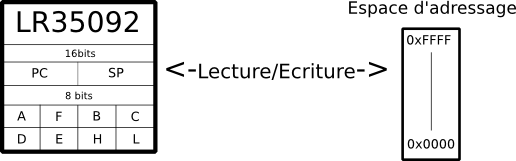
\includegraphics[scale=0.80]{images/schema_cpu.png}
\caption{Schéma représentant le LR35902}
\end{figure}
\section{GPU}

Le GPU de la Game Boy est intégré dans le même circuit physique que le CPU. Sa fonction est de générer une image à partir des données contenues dans la VRAM (vidéo ram) puis de l'envoyer à l'écran LCD, il possède différents registres de configuration.

\subsection{Fonctionnement de l'écran}

L'affichage de la Game Boy se fait via un écran LCD d'une résolution de 160*144 pixels. Cet affichage se fait en périodes, il va tout d'abord afficher une ligne puis passer dans une période dite de HBlank, ce qui correspond à un retour à la ligne, puis afficher la ligne suivante. Cette routine s'effectue jusqu'à la ligne 144, s'ensuit alors une période de VBlank qui correspond à un retour à la première ligne.
Ces périodes de VBlank ou de HBlank ont un nombre de cycles défini, c'est
durant ces périodes que l'accès aux différentes matrices en écriture va être
débloqué pour que le CPU puisse modifier les éléments à afficher.\\\\

\begin{figure}[!h]
\centering
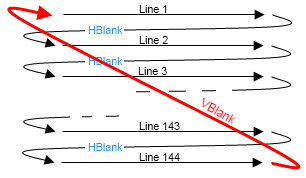
\includegraphics[scale=0.8]{images/gpu_cycles.png}
\caption{Schéma des cycles d'affichage du GPU}
\label{gpucycles}
\end{figure}


\subsection{Génération d'une ligne}

Trois types de couches graphiques peuvent être affichées: la couche background, la couche
window et la couche sprites, les deux premières peuvent être activées ou
désactivées selon les jeux en modifiant un registre ( à l'adresse FF40 ).

Ces trois couches ont des rôles différents et servent à séparer différents
éléments graphiques d'un jeu.\\

\begin{itemize}
\item \textbf{La couche Background:}
	Cette couche comprend tous les éléments qui appartiennent au décor du
jeu. Elle est représentée par deux matrices de 256*256 pixels, soit 32*32
tuiles (carrés de 8*8 pixels). La Game Boy peut donc passer d'une matrice à
l'autre pour réaliser des transitions vidéos entre deux scènes. Ces matrices étant
d'une taille supérieure à celle de l'écran lors de l'affichage, il est possible de gérer la position de
l'écran sur une zone desdites matrices via la modification des valeurs de
deux registres. 
\\
\item \textbf{La couche Window:}
	Cette couche est généralement utilisée pour tous les éléments statiques
d'un jeu, comme la barre de menu ou les scores. Elle a un comportement
similaire à celui de la couche Background si ce n'est qu'elle est positionnée par rapport à l'écran et non l'inverse.\\

\item \textbf{La couche Sprites:}
	Cette couche est utilisée pour représenter les éléments mobiles d'un jeu (personnages, objets, etc). Elle est représentée en mémoire par un maximum
de 40 tuiles différentes. Ces tuiles sont positionnées à l'écran via un registre indiquant leur position absolue, ainsi que diverses options d'affichage, comme la possibilité d'appliquer une symétrie verticale ou horizontale sur la tuile.\\
\end{itemize}

\subsection{Les couleurs}

Les couches Background et Window utilisent un registre (palette monochrome) pour gérer les
couleurs des différents pixels, dans le cas de la Game Boy ce registre contient
4 niveaux de gris codés sur 2 bits.

La couche Sprite peut utiliser deux palettes qui diffèrent en un point de la précédente : la valeur 00 ne correspond pas au blanc mais au fait que
le pixel soit transparent.\\

\subsection{Les registres d'affichage}
\subsubsection{LCD Control Register}
C'est un registre 8 bits accessible en lecture et écriture situé à l'adresse 0xFF40, il permet de gérer les principales options d'affichage de l'écran LCD:\\

\begin{itemize}
\item \textbf{bit 0:}
	Permet de gérer l'affichage du Background, mis à 0 il permet d'afficher un fond blanc à la place du Background. Mis à 1 le Background sera affiché normalement.\\
\item \textbf{bit 1:}
	Permet l'affichage ou non des sprites.\\
\item \textbf{bit 2:}
	Ce bit indique la taille des sprites utilisés. S'il est mis à 0, des sprites de 8*8 seront utilisés, par contre s'il est mis à 1 les sprites auront une taille de 8*16.\\
\item \textbf{bit 3:}
	Ce bit permet de choisir quelle matrice de tuiles à utiliser pour afficher le Background. Mis à 0, la matrice située entre 0x9800 et 0x9BFF sera utilisée, à 1 la matrice située entre 0x9C00 et 0x9FFF sera utilisée.\\
\item \textbf{bit 4:}
	Même fonctionnement que le bit précédent sauf que celui-ci sert à choisir la matrice contenant les données des tuiles. La matrice contenue entre les adresses 0x8800 et 0x97FF est choisie si le bit est à 0, sinon c'est celle entre les adresses 0x8000 et 0x8FFF.\\
\item \textbf{bit 5:}
	Permet de gérer l'affichage de la couche Window. Si 0 elle n'est pas affichée, si 1 elle l'est.\\
\item \textbf{bit 6:}
	Même fonctionnement que le bit 3 sauf qu'il permet de choisr la matrice de tuiles pour afficher la Window.\\
\item \textbf{bit 7:}
	Ce bit sert à activer ou désactiver l'écran LCD. Il doit être désactivé seulement pendant les périodes de VBlank sous peine d'endommager la Game Boy. Mettre à 0 ce bit rend aussi accessible librement la VRAM et OAM.\\
\end{itemize}

\subsubsection{LCD Status Register}
Ce registre 8 bits est accessible en lecture et écriture, il est situé à l'adresse 0xFF41 et permet de gérer les interruptions liées au GPU:\\

\begin{itemize}
\item \textbf{bit 0-1}
	Ces bits correspondent au Mode Flag et sont accessibles seulement en lecture. Ils déterminent dans quelle période l'écran LCD se trouve: 0 pour le HBlank, 1 pour le VBlank, 2 pour la lecture de la mémoire OAM et 3 pour le transfert des données vers l'écran LCD.\\
\item \textbf{bit 2:}
	Accessible seulement en lecture, il représente le "Coincidence Flag", il est mis à 0 si les registres LYC et LY sont différents, à 1 sinon.\\
\item \textbf{bit 3:}
	Ce bit est mis à 1 si une interruption liée au HBlank est nécessaire.\\
\item \textbf{bit 4:} 
	Idem que le bit précédent mais pour le VBlank.\\
\item \textbf{bit 5:}
	Idem mais pour la mémoire OAM.\\
\item \textbf{bit 6:}
	Ce bit est activé si la valeur du registre LYC et celle du registre LY sont égales, une interruption sera alors déclenchée.\\
\item \textbf{bit 7:}
	Il n'est pas utilisé.\\
\end{itemize}

\subsection{OAM}
	La table OAM (Object Attribute Memory) est située entre les adresses 0xFE00 et 0xFE9F, elle contient tous les attributs liés aux sprites. Elle est accessible uniquement pendant les périodes de HBlank et de VBlank. Elle est composée de 40 entrées de 4 octets chacunes:\\

\begin{itemize}
\item \textbf{octet 0:}
	Cet octet spécifie la position verticale du sprite, qui sera invisible si sa position dépasse la largeur de l'écran.\\
\item \textbf{octet 1:}
	Cet octet spécifie la position horizontale du sprite, les valeurs doivent être comprises entre 8 et 168 pour qu'il soit visible.\\
\item \textbf{octet 2:}
	Cet octet correspond à la position d'une tuile dans la matrice qui les contient toutes, située entre 0x8000 et 0x8FFF.\\
\item \textbf{octet 3:}
	\begin{itemize}
	\item \textbf{bit 0-3:}
		Utilisés uniquement pour la Game Boy Color.\\
	\item \textbf{bit 4:}
		Permet de choisir laquelle des deux palettes de couleurs est à utiliser.\\
	\item \textbf{bit 5:}
		S'il est activé, applique une symétrie horizontale sur le sprite.\\
	\item \textbf{bit 6:}
		S'il est activé, applique une symétrie verticale sur le sprite.\\
	\item \textbf{bit 7:}
		Ce bit indique qui, du sprite ou de la couche Background est prioritaire sur l'affichage. \\
	\end{itemize}
	
\end{itemize}

\subsection{VRAM}
La VRAM correspond à la RAM vidéo de la Game Boy, sa taille est de 8 KBytes. Elle est donc utilisée pour tout ce qui touche à l'affichage, qu'il s'agisse des nuances de gris ou des différentes couches d'affichage. Tous les registres que nous avons vu précédemment sont contenus en son sein.
	


\section{MMU}
Le MMU (soit Memory Management Unit) est un composant qui autorise ou non l'accès en mémoire demandé par le processeur.
En fait la Game Boy ne possède pas de tel composant, seulement le processeur est bien raccordé directement à un espace d'adressage de 16 bits.
Pour mieux comprendre à quoi correspond cet espace, l'espace d'adressage sera
dans un premier temps découpé grossièrement, puis chaque partie sera étudiée
plus en détails:\\
\begin{itemize}
\item \textbf{0xFE00-0xFFFF} Espace mémoire particulier
\item \textbf{0xC000-0xFDFF} RAM interne
\item \textbf{0xA000-0xBFFF} RAM de la cartouche
\item \textbf{0x8000-0x9FFF} RAM interne dédiée aux dessins du jeu
\item \textbf{0x0000-0x7FFF} ROM de la cartouche
\end{itemize}

\subsection{0x0000-0x7FFF ROM de la cartouche}
\begin{itemize}
\item \textbf{0x0000-0x3FFF:} Banque 0 de la ROM de la cartouche.
\item \textbf{0x4000-0x7FFF:} Banque 1-n de la ROM de la cartouche (voir partie Cartouche de jeu).
\end{itemize}

\subsection{0x8000-0x9FFF RAM interne dédiée aux dessins du jeu}
\begin{itemize}
\item \textbf{0x8000-0x97FF:} Données des dessins, où sont stockés tous les dessins du jeu.
\item \textbf{0x9800-0x9BFF:} "Background Map" 1, zone spécifiant les dessins à utiliser pour dessiner l'arrière-plan 1.
\item \textbf{0x9C00-0x9FFF:} "Background Map" 2, zone spécifiant les dessins à utiliser pour dessiner l'arrière-plan 2. 
\end{itemize} 

\subsection{0xA000-0xBFFF RAM de la cartouche}
Zone dédiée à la RAM de la cartouche (Voir Partie Cartouche de jeu).

\subsection{0xC000-0xFDFF RAM interne}
\begin{itemize}
\item \textbf{0xC000-0xDFFF:} Zone de RAM interne servant à stocker les différentes variables du jeu.
\item \textbf{0xE000-0xFDFF:} Echo de la plage d'addresse de 0xC000 à 0xDDFF, cette zone est
généralement inutilisée.
\end{itemize} 

\subsection{0xFE00-0xFFFF Espace mémoire particulier}

\begin{itemize}
\item \textbf{0xFE00-0xFE9F:} Object Attribute Memory (OAM), zone contenant les informations
sur les sprites affichés.
\item \textbf{0xFEA0-0xFEFF:} Inutilisé.
\item \textbf{0xFF00-0xFF7F:} Cette zone contient des registres de contrôles pour tous les composants de la
Game Boy.
\item \textbf{0xFF80-0xFFFE:} Cette zone est réservée pour la pile, les
développeurs initialisent généralement le registre SP à l'adresse 0xFFFE.
\item \textbf{0xFFFF :} Cette adresse sert à savoir quelles interruptions sont autorisées ou
non. (Voir partie Interruptions)
\end{itemize} 

\section{Cartouche de jeu}
Une cartouche de jeu est composée au minimum d'une mémoire morte, appelée ROM (Read Only Memory), mais peut aussi contenir dans certains cas de la RAM (Random Access Memory) ou d'autres composants que nous verrons un peu plus loin.

\subsection{Le header}
Dans chaque cartouche, une zone d'information la concernant est située entre les adresses 0x0100 et 0x014F, cette zone est appelée le header. Les différentes informations contenues dans cette zone sont les suivantes:\\

\begin{itemize}

\item \textbf{0x0100-0x0103:} Cette adresse est le point d'entrée du programme. Après l'affichage du logo Nintendo, le processeur exécute un "jump" vers cette adresse, puis un second vers la valeur qu'elle contient qui est en fait celle du début du programme.\\

\item \textbf{0x0104-0x0133:} Cette addresse contient les octets définissant le logo Nintendo quand la Game Boy s'allume. Les valeurs sont les suivantes:
\\CE ED 66 66 CC 0D 00 0B 03 73 00 83 00 0C 00 0D
\\00 08 11 1F 88 89 00 0E DC CC 6E E6 DD DD D9 99
\\BB BB 67 63 6E 0E EC CC DD DC 99 9F BB B9 33 3E\\

\item \textbf{0x0134-0x0143:} Le titre du jeu est stocké à cette adresse, il est écrit en majuscule et en ASCII.\\

\item \textbf{0x013F-0x0142:} Cette adresse correspond au code de l'entreprise qui a créé le jeu, par exemple pour Nintendo, cette adresse aura la valeur 0x33.\\

\item \textbf{0x0143:} Le CGB (Color Game Boy) Flag est contenu à cette adresse, il permet d'indiquer si le jeu est compatible avec les autres Game Boy ou seulement avec la Game Boy Color.\\

\item \textbf{0x0144-0x0145:} Cette adresse contient deux caractères ASCII qui indiquent la société ayant publié le jeu.\\

\item \textbf{0x0146:} Le SGB (Super Game Boy) Flag est stocké ici, il permet de savoir si le jeu est compatible avec les fonctionnalités de la SGB.\\

\item \textbf{0x0147:} Cette adresse spécifie quel MBC (Memory Bank Controller) est utilisé par la cartouche et si il y a des composants externes comme une batterie ou une caméra. Nous aborderons cette partie un peu plus loin.\\

\item \textbf{0x0148:} La taille de la ROM est indiquée à cette adresse:
\\00h -  32KByte (pas de banque)
\\01h -  64KByte (4 banques)
\\02h - 128KByte (8 banques)
\\...

\item \textbf{0x0149:} La taille de la RAM est indiquée à cette adresse:
\\00h - Aucune
\\01h - 2 KBytes
\\02h - 8 Kbytes
\\03h - 32 KBytes\\

\item \textbf{0x014A:} Cette adresse contient le code qui indique si le jeu est censé être vendu au Japon ou ailleurs.\\

\item \textbf{0x014D:} Le Header Checksum est contenu ici. Lors du lancement d'un jeu si les 8 bits de poids faible du résultat du checksum ne sont pas égaux à ceux contenus à cette adresse , le jeu ne se lancera pas.\\

\end{itemize}

\subsection{Memory Bank Controllers}
Les bus d'adressage de 16 bits de la Game Boy offrent un espace d'adressage limité pour la ROM et la RAM. De ce fait, la plupart des cartouches utilisent une puce nommée MBC qui permet d'étendre cet espace en changeant de banque. Les différents types de puces MBC utilisés par la Game Boy sont les suivants:\\

\subsubsection{MBC1}
	La puce MBC1 est la première puce MBC, toutes les suivantes fonctionnent de manière similaire, ce qui permet une compatibilité et une mise à niveau relativement simple. Cette puce est utilisée par les jeux ne dépassant pas 2MByte de ROM et/ou 32 KByte de RAM.

La répartition des adresses est la suivante:\\
\begin{itemize}
\item \textbf{0x0000-0x3FFF:} La banque de ROM 00 , cette banque contient toujours les 16 premiers KBytes de la ROM de la cartouche.\\
\item \textbf{0x4000-0x7FFF:} Les banques de ROM 01 à 7F, cette zone contient toutes les autres banques de 16 KBytes, ce qui correspond à un total de 125 banques utilisables car les banques 0x20, 0x40 et 0x60 ne sont pas accessibles.\\
\item \textbf{0xA000-0xBFFF:} Les banques de RAM 00 à 03 si elles existent. La RAM de la cartouche est principalement utilisée en complément d'une batterie pour pouvoir stocker les scores ou les sauvegardes et cela même si la Game Boy est éteinte ou la cartouche retirée.\\
\item \textbf{0x0000-0x1FFF:} Cette adresse permet d'autoriser ou d'interdire l'écriture dans la RAM. Y écrire la valeur 0x0A permet d'autoriser l'écriture et 0x00 de l'interdire.\\
\item \textbf{0x2000-0x3FFF:} Ecrire à cette adresse permet de sélectionner une banque. La banque est sélectionnée en fonction des 5 bits de poids faible, par contre si 0x00 est écrit la banque sélectionnée sera la banque 01, la même chose se passe pour les banques 20, 40 et 60.\\
\item \textbf{0x4000-0x5FFF:} Ce registre de 2 bits permet de sélectionner une banque de RAM. Suivant le mode sélectionné (voir plus bas) il pourra aussi servir à sélectionner les 2 bits de poids fort de la banque de ROM.\\
\item \textbf{0x6000-0x7FFF:} Ce registre de 1 bit va permettre de savoir comment vont être utilisés les 2 bits du registre précédent. Si la valeur 0x00 s'y trouve, ils sont utilisés pour choisir la banque de ROM, de RAM pour 0x01.\\
\end{itemize}
\subsubsection{MBC2}
	La puce MBC2 est une version améliorée de la puce précédente, elle est utilisée par les jeux ayant au plus 256 KByte de ROM et 4x512 bits de RAM.
\\Les différences entre les deux puces sont les suivantes:\\
\begin{itemize}
\item \textbf{0x4000-0x7FFF:} Même chose que la précédente sauf qu'un total de 16 banques de ROM est supporté.\\
\item \textbf{0A000-A1FF:} Le MBC2 n'étant pas compatible avec la RAM externe, 512*4 bits de RAM sont inclus directement dans la puce du MBC, ce qui requiert une batterie pour sauvegarder les données durant les périodes où la Game Boy est éteinte.\\
\item \textbf{0x0000-0x1FFF:} Cette adresse permet d'activer ou de désactiver la RAM.\\
\item \textbf{0x2000-0x3FFF:} Les 4 bits de poids faible écrits ici servent à sélectionner la banque de ROM.\\
\end{itemize}
\subsubsection{MBC3}
	La puce MBC3 est la dernière version de la puce MBC1, compatible avec la Game Boy, elle est principalement utilisée par les jeux prenant en compte l'heure actuelle et donc ayant besoin d'une horloge interne à la cartouche.\\
La plupart des registres fonctionnent de la même façon que son ancêtre, à quelques détails techniques près, les suivants permettant d'ajouter les fonctionnalités de gestion du temps.
\begin{itemize}
\item \textbf{0xA000-0xBFFF:} Cet espace est utilisé pour accéder à une banque de RAM externe ou au registre d'horloge.\\
\item \textbf{0x6000-0x7FFF:} Faire basculer la valeur de ce registre permet de verrouiller ou déverrouiller l'heure actuelle dans les registres d'horloge.\\ 
\end{itemize}

\subsubsection{Aucun}
	Les petits jeux qui ne dépassent pas 32 KBytes de ROM ne requièrent pas de puce MBC. La ROM est directement répartie sur les adresses 0x0000 à 0x7FFF et la RAM de 0xA000 à 0xBFFF. Ces jeux contiennent tout de même une petite puce semblable à une MBC.\\

\section{APU}
\subsection{Présentation générale}
	La Game Boy dispose de deux canaux de son (un pour la gauche,
	et un pour la droite), reliés aux terminaux de sortie appelés
	SO1 et SO2 par le constructeur, ainsi que d'un terminal
	d'entrée appelé Vin, recevant le signal électrique
	correspondant au son de la cartouche et pouvant être redirigé après
	traitement vers le terminal SO1, SO2, ou les deux en même
	temps (pour passer d'un son mono à un son stéréo par
	exemple).
\begin{figure}[!h]
\centering
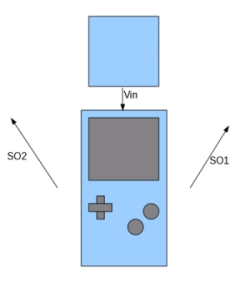
\includegraphics[scale=0.5]{images/GBSound1.jpg}
\caption{Le son Game Boy : entrées et sorties}
\label{GBS1}
\end{figure}

	Grossièrement, les composants de l'appareil permettent de
	créer un son de quatre façons différentes : 
		\begin{itemize}
		\item Une première onde carrée, avec une enveloppe de
		volume et une fonction de balayage.
		\item Une seconde onde carrée avec enveloppe de volume
		aussi mais sans fonction de balayage.
		\item Une onde formée à partir d'échantillons
		prédéfinis et stockés en mémoire cartouche.
		\item Et une onde "Bruit" avec une enveloppe de
		volume.
		\end{itemize}
	Ces quatre ondes sont générées indépendamment et finalement
	"mixées" pour diriger vers les canaux de sortie celle
	correspondant au son à produire pour le jeu.

\subsection{Registres, valeurs et contrôles} 
	Pour générer cette musique sans laquelle les jeux n'auraient
	sûrement pas la même dimension, la console dispose de 22
	registres, qu'elle peut consulter et modifier à quasiment
	n'importe quel moment dès lors que le son du jeu à commencé à
	être joué.\\
	Ces registres sont séparés en 5 "familles" (4 pour les quatre
	ondes, et une pour les contrôles du son) numérotés et appelés
	par convention \textbf{NRXX} où NR signifie "Noise Register", et XX le
	numéro dudit registre. \\
	Chacun de ces registres peut être utilisé pour stocker une
	ou plusieurs valeurs, en utilisant tout ou seulement une
	partie des 8 bits qu'il contient.\\

	NB : La notation "bits 0 à x" (x = 5 par exemple) signifie
	plus exactement la valeur binaire que l'on obtient en
	extrayant lesdits bits du registre et en les traitant comme un
	nouveau nombre.\\
	Par exemple pour une valeur lue de 01101011 dire "les bits 4 à
	6 donnent la valeur d'un volume" correspond à dire "le nombre binaire
	110 donne la valeur d'un volume".

	\subsubsection{Son et balayage}
	La première famille comporte cinq registres, utilisés pour
	générer et modifier le premier type d'onde, les ondes carrées
	avec enveloppe de volume et fonction de balayage.\\

	\textbf{NR10(FF10):} le registre de balayage.\\
		C'est le premier exemple de registre utilisé pour
		stocker plusieurs valeurs, ici les bits 4 à 6 donnent
		la valeur de la fréquence de balayage, les bits 0 à 2
		le nombre de décalage de ces balayages à effectuer, et le bit
		numéro 3 indique par sa valeur (0 ou 1) s'il s'agit
		d'un balayage montant (où la fréquence augmente) ou
		d'un balayage descendant (où elle diminue).\\ 
	
	\textbf{NR11(FF11):} Forme d'onde et longueur de son\\
		Les bits 4 à 6 de ce registre contiennent la valeur de
		forme d'onde, chacune des 4 valeurs possibles donne
		une valeur de "temps montant" (1/8 pour 0, 1/4 pour
		1, 1/2 pour 2 et 3/4 pour 3).
		Les bits 0 à 5 donnent la valeur de la longueur
		du son à jouer. Cette valeur n'est prise en
		compte que si c'est indiqué dans le registre \textbf{NR14}.\\
	
	\textbf{NR12(FF12):} Enveloppe de volume \\
		Les bits 4 à 7 donnent la valeur initiale de volume de
		l'enveloppe.
		Le bit numéro 3 indique la "direction" de l'enveloppe,
		à savoir si le son sera lu avec un volume augmentant
		ou descendant.
		Les bits 0 à 2 donnent la valeur d'un nombre
		d'utilisation de l'enveloppe.\\ 
	
	\textbf{NR13(FF13):} Composantes basses de la fréquence \\
		La fréquence du son à jouer est un nombre sur 11 bits
		dont les 8 représentant la composante basse sont
		stockés ici et les 3 manquants représentant la
		composante haute sont stockés dans le registre
		suivant.\\ 

	\textbf{NR14(FF14)}: Composantes hautes \\
		Le bit 7 est un indicateur de ré-initialisation de la
		fréquence, le bit 6 un compteur d'opérations
		consécutives, qui va indiquer si la longueur lue sur
		les bits 0 à 5 du registre \textbf{NR11} est à prendre en
		compte ou non, et les bits 0 à 2 contiennent les 3 bits
		manquant à la fréquence stockée en \textbf{NR13}.
	\subsubsection{Son}
		La deuxième famille correspond à la deuxième onde carrée, elle
		fonctionne comme la première mais sans le registre de
		balayage. Le fonctionnement, l'ordre et les valeurs des bits
		correspondent aux mêmes descriptions que pour la première
		famille, la seule différence réside dans les registres
		utilisés.\\ \\
	
	Le registre \textbf{NR21(FF16)} fonctionne comme le \textbf{NR11} (à
		l'exception de la vérification de prise en compte de
		la longueur, qui se fait via le bit 6 du registre \textbf{NR24}
		cette fois ci), le \textbf{NR22(FF17)} fonctionne comme le
		\textbf{NR12}, le \textbf{NR23(FF18)} fonctionne comme le \textbf{NR13} et le
		\textbf{NR24(FF19)} comme le \textbf{NR14}. 
			
	\subsubsection{Onde mémoire}
		Cette famille de registres correspond principalement à
		l'utilisation de sons pré-enregistrés dans la cartouche
		(et certains dans la Game Boy, le bruit de démarrage par
		exemple).
		Dans certains cas elle peut être utilisée pour jouer un son de
		la même façon que les 2 premières ondes, ce qui explique la
		présence des registres \textbf{NR33} et \textbf{NR34}. \\ 
		
	\textbf{NR30(FF1A):} Trigger de son \\ 
		Il n'est utilisé que pour indiquer via la
		valeur du bit 7 si l'onde mémoire est à utiliser ou
		non.\\
		
	\textbf{NR31(FF1B):} Longueur de son \\
		La valeur entière (bits 0 à 7) du
		registre est utilisée et donne la longueur du son à
		jouer.\\ 
		
	\textbf{NR32(FF1C):} Sélecteur \\
		Les bits 5 à 6 donne la valeur d'un
		sélecteur de volume pour le son à jouer, il est joué
		sans son pour une valeur de 0, tel quel pour 1, avec un volume à 50pourcents 
		pour 2 (décalé d'un bit vers la droite), et un volume
		de 25pourcents pour 3 (décalé de deux bits vers la droite). \\
		
	\textbf{NR33(FF1D):} Composantes basses \\
		Comme pour les \textbf{NR13} et \textbf{NR23}, ce registre
		contient les 8 premiers bits de la valeur de fréquence
		du son à jouer.\\

	\textbf{NR34(FF1E):} Composantes hautes \\
		Celui-ci fonctionne comme les \textbf{NR14} et \textbf{NR24} mais pour
		cette 3ème onde (utilisé dans le cas d'une utilisation
		de cette onde pour produire un son sans utiliser les
		sons mémoire). \\

	Les registres \textbf{FF30} à \textbf{FF3F} ne sont pas numérotés en NR
		mais contiennent les sons pré-enregistrés à jouer, ils
		sont stockés sous la forme de 32 échantillons de 4
		bits chacun, soit 16 valeurs 8 bits lues dans l'ordre
		4 bits de poids fort en premier et 4 bits de poids
		faible ensuite.

	\subsubsection{Bruit}
		Cette famille de registre correspond à une onde de son
		appelé "bruit blanc", c'est généralement d'elle que
		vienne les sont saturés que l'on entend dans la
		plupart des jeux (une brique cassée dans Super Mario
		par exemple!). 
		Ce bruit est réalisé par une variation aléatoire
		d'amplitude entre composantes hautes et basses d'une
		fréquence donnée. Le son paraîtra plus ou moins rude
		en fonction de cette fréquence. \\
		Cette onde est aussi parfois utilisée pour générer un
		son correct en régularisant la sortie par une
		modification volontaire de la modification aléatoire
		d'amplitude (qui par conséquent, n'est plus réellement
		due au hasard). \\

	\textbf{NR41(FF20):} Longueur de son \\
		Les bits 0 à 5 donnent la valeur de la longueur du son
		à jouer.\\

	\textbf{NR42(FF21):} Enveloppe de volume\\
		Les bits 4 à 7 correspondent à la valeur initiale de
		l'enveloppe, le bit numéro 3 donne sa direction
		(montante ou descendante) et les bits 0 à 2 donnent le
		nombre d'utilisations de l'enveloppe.\\

	\textbf{NR43(FF22):} Compteur polynomial \\
		L'amplitude est modifiée aléatoirement entre haute et
		basse sur la fréquence donnée. Plus cette fréquence
		est haute, moins le bruit paraîtra rude. 
		Si le bit 3 est activé, l'intervalle de valeurs
		aléatoires est réduit, et la sortie devient plus
		régulière, la rendant la plus proche d'un réel
		son que d'un bruit (au sens physique du terme).
		Les bits 4 à 7 donnent la fréquence utilisée, le bit 3
		indique la taille de l'intervalle des valeurs
		aléatoires d'amplitude et les bits 0 à 2 correspondent
		à une valeur de diviseur de fréquence.\\ 

	\textbf{FF23(NR43):} Compteur consécutif\\
		Le bit 7 est un initialisateur, il réinitialise le bruit
		lorsque sa valeur est 1.
		Le bit 6 est l'indicateur de jeu du son, il indique
		qu'il faut stopper en passant à 0 lorsque la valeur de
		longueur du son lue en \textbf{NR41} tombe à 0. 
	\subsubsection{Contrôles du son}
		C'est la cinquième et ultime famille de registres
		utilisés pour produire du son avec la console, elle
		correspond à un ensembles de registres dont les
		valeurs servent à contrôler physiquement dans son
		ensemble, par exemple indiquer le canal de sortie,
		gérer le volume général ou simplement activer ou
		désactiver le son de la console. \\

	\textbf{NR50(FF24):} Contrôle du signal d'entrée \\ 
		Le bit 7 envoie le signal Vin vers la sortie SO2
		lorsqu'il est activé, alors que le bit 3 l'envoie vers
		la sortie SO1. les bits 6 à 4 correspondent au volume
		propre à la SO2, et les 0 à 2 à celui de la SO1. \\

	\textbf{NR51(FF25):} Sélection du terminal de sortie propre \\
		Ici les bits redirigent les 4 ondes possibles vers un
		terminal donné.
		Les bits 0 à 3 envoie respectivement les ondes 1 à 4
		vers la SO1, les bits 4 à 7 envoie respectivement les
		ondes 1 à 4 vers la SO2.\\

	\textbf{NR52(FF26):} Activation du son \\
		Les bits 0 à 3 de ce registre activent (ou
		désactivent) respectivement les ondes 1 à 4 et le bit
		7 indique si le son général de la console est activé
		ou non.
\section{Interruptions/Synchronisations}
Comme vu dans les parties précédentes, le processeur de la Game Boy travaille conjointement avec d'autres composants. Afin d'éviter un chaos général voire l'endommagement de certains composants, un système d'interruptions a été intégré dans l'architecture de la Game Boy.
\subsection{Que fait une interruption?}
Lorsqu'une interruption est déclenchée, le processeur va interrompre ses calculs afin d'exécuter une routine. Pour cela le processeur va ajouter dans la pile le registre PC et remplacer la valeur du registre PC par l'adresse de la routine. L'adresse de la routine est différente selon le type d'interruption déclenchée.
\subsection{Registres d'interruption}
Afin qu'une interruption soit déclenchée il faut qu'un certain nombre de conditions soient réunies.
\subsubsection{Registre IME}
En premier lieu le processeur dispose d'un registre spécial appelé IME (Interrupt Master Enabled), qui va contrôler si les interruptions peuvent être déclenchées ou non. Si IME est à 0 aucune interruption ne sera déclenchée, sinon si IME est à 1 les interruptions peuvent être déclenchées.
\subsubsection{Registres IE et IF} 
IE correspond à 'Interrupt Enable' et IF correspond à 'Interrupt Flag', ces deux registres sont stockés en mémoire. IE est disponible à l'adresse 0xFFFF et IF à l'adresse 0xFF0F. Le registre IE signale quelles interruptions peuvent être déclenchées. Le registre IF signale quelles interruptions veulent être déclenchées.
Comme il existe cinq types d'interruptions, cinq bits de ces registres vont servir à savoir quelle interruption est demandée/activée:\\\\
\textbf{0xFFFF - IE - Interrupt Enable} \\
Bit 0: V-Blank  Interruption Autorisée  (1=Autorisée)\\
Bit 1: LCD STAT Interruption Autorisée  (1=Autorisée)\\
Bit 2: Timer    Interruption Autorisée  (1=Autorisée)\\
Bit 3: Serial   Interruption Autorisée  (1=Autorisée)\\
Bit 4: Joypad   Interruption Autorisée  (1=Autorisée)\\\\
\textbf{0xFF0F - IF - Interrupt Flag} \\
Bit 0: V-Blank  Requête d'Interruption  (1=Requête)\\
Bit 1: LCD STAT Requête d'Interruption  (1=Requête)\\
Bit 2: Timer    Requête d'Interruption  (1=Requête)\\
Bit 3: Serial   Requête d'Interruption  (1=Requête)\\
Bit 4: Joypad   Requête d'Interruption  (1=Requête)\\\\

\subsection{Quand est-ce qu'une interruption est déclenchée?}
Pour qu'une interruption soit déclenchée, par exemple l'interruption VBlank, Il faut que IME soit à 1, et que les bits 0 de IE et IF soit à 1 également.
Lorsqu'elle sera déclenchée le bit 0 de IF sera mis à 0. IME sera mis à 0 également pour éviter qu'une interruption soit déclenchée pendant la routine d'une autre interruption (bien que cela soit possible pour le développeur en utilisant l'instruction "EI" dans une routine d'interruption).
\subsection{Les différents types d'interruptions}
\subsubsection{Interruption VBlank}
L'interruption VBlank est demandée par l'écran LCD, cette demande est faite à chaque fois que l'écran rentre dans la période de VBlank (Voir partie GPU), l'interruption sert généralement à mettre à jour les dessins du jeu avant l'affichage d'une nouvelle image. La routine se trouve à l'adresse 0x0040.
\subsubsection{Interruption LCD STAT}
Cette interruption est également demandée par l'écran LCD, elle sert généralement à exécuter des routines lorsque l'écran LCD change d'état (Voir partie GPU). Elle peut aussi intervenir lorsque la ligne actuellement dessinée par l'écran LCD correspond au registre LYC (LY compare). la routine se trouve à l'adresse 0x0048.
\subsubsection{Interruption Timer}
Interruption générée par le timer interne de la Game Boy, à chaque fois que celui-ci dépasse une certaine durée. La routine se trouve à l'adresse 0x0050.
\subsubsection{Interruption Serial}
Interruption générée lorsqu'un transfert d'un octet à été fait (reçu ou transmis) à l'aide du câble Link servant à communiquer entre deux Game Boy ou entre une Game Boy et un ordinateur. La routine se trouve à l'adresse 0x0058.
\subsubsection{Interruption Joypad}
Interruption générée lors de l'appui sur une touche par le joueur. La routine se trouve à l'adresse 0x0060.
\section{Autres composants}
La Game Boy comprend d'autres composants tels un timer interne, ou un port appelé "link" permettant de communiquer avec une autre Game Boy. Ces composants ne seront pas détaillés, en raison pour le timer du fait que son mécanisme est assez simple et dispensable pour la compréhension du fonctionnement général d'un émulateur. Pour le port link bien que ce composant soit très intéressant nous n'avons pas eu le temps, à notre regret, de nous y pencher et de l'implémenter.
\chapter{Réalisation}
Ce chapitre synthétise la manière dont nous avons réalisé groboy, notre émulateur.
\section{CPU}
Le processeur a été le premier "composant" à être développé. Nous allons donc décrire dans cette partie comment il a été réalisé.
\subsection{Structure}
En premier lieu nous avons défini une structure rassemblant tous les registres utilisés par le processeur.
Voici sa forme:
\begin{lstlisting}
typedef struct {
	unsigned short PC;
	unsigned short SP;
	unsigned char A;
	unsigned char F;
	unsigned char B;
	unsigned char C;
	unsigned char D;
	unsigned char E;
	unsigned char H;
	unsigned char L;	
} z80_t;
\end{lstlisting}
On retrouve bien tous les registres ainsi que leur taille respective, à noter que nous avons préféré l'appeler z80\_t au lieu de lr35902\_t par commodité.
\subsection{Algorithme principal}
Une fois la structure définie nous avons mis en place un algorithme servant de "base" au comportement de notre CPU. Pour cela nous nous sommes largement inspiré des conseils de la page de KomKon\cite{komkon}. Voici son allure générale:
 \begin{lstlisting}
void run(){
	BYTE op_code;
	for(;;)
	{
		op_code = memory_read(z80.PC++);
		cycles = z80_cycles[op_code];
		switch(op_code){	
			case 0x00:
				//Appel de l'opcode 0x00.
				break;
			case 0x01:
				//Appel de l'opcode 0x01.
				break;
			...
			case 0xFF:
				//Appel de l'opcode 0xFF.
				break;
		}
		update_other_components(cycles);
		handle_interrupts();
	}
}
 \end{lstlisting}		
Ici plusieurs choses interviennent, nous allons détailler chacune de ces choses.
\begin{lstlisting}
for(;;){
	...
}
\end{lstlisting}
Le processeur est un composant qui travaille sans relâche jusqu'à sa mise hors tension, d'où la boucle infinie. On préférera déclarer la boucle infinie de cette manière plutôt qu'avec un simple "while(1)" évitant à certains compilateurs de faire vérifier la condition.
\begin{lstlisting}
op_code = memory_read(z80.PC++);
\end{lstlisting}
Pour pouvoir lire la prochaine instruction à exécuter, nous avons implémenté une fonction memory\_read, cette fonction a la signature suivante:
\begin{lstlisting}
unsigned char memory_read(unsigned short addr);
\end{lstlisting}
En fait cette fonction retourne la valeur située en mémoire à l'adresse "addr", comme dit précédemment dans la section MMU. Le processeur à une plage d'adresses de 16 bits, d'où le type unsigned short de la variable addr.
Vous vous en doutez alors, nous avons également implémenté une fonction pour écrire en mémoire. Sa signature est:
\begin{lstlisting}
void memory_write(unsigned short addr, unsigned char data);
\end{lstlisting}

\begin{lstlisting}
cycles = z80_cycles[op_code];
\end{lstlisting}
Comme décrit dans la section Hardware-CPU chaque instruction a un nombre de cycles représentant son coût en temps. Cette ligne sert à récupérer dans le tableau "z80\_cycles" ce nombre de cycles.
\begin{lstlisting}
switch(op_code){	
	case 0x00:
		//Appel de l'opcode 0x00.
		break;
	case 0x01:
		//Appel de l'opcode 0x01.
		break;
	...
	case 0xFF:
		//Appel de l'opcode 0xFF.
		break;
}
\end{lstlisting}
Ici est la partie où l'instruction va être exécutée, un switch est mis en place sur la valeur de l'instruction. Lorsqu'il y'a beaucoup de cas différents il est toujours préférable de faire un switch géant, plutôt qu'une suite de "if, else if", car au niveau de l'exécutable le switch permet d'aller directement sur la bonne valeur grâce à l'instruction "jump". Une suite de "if, else if" nécessite de vérifier chacune des valeurs jusqu'à trouver la bonne. 
\begin{lstlisting}
update_other_components(cycles);
\end{lstlisting}
Cette fonction donne aux autres composants le nombre de cycles exécutés pour qu'ils puissent être synchronisés avec le processeur et pour qu'ils fassent leurs routines.
\begin{lstlisting}
handle_interrupts();
\end{lstlisting}
Enfin, après les routines des autres composants, il se peut qu'il y'ait une interruption déclenchée, c'est le rôle de cette fonction, de voir si une interruption a été déclenchée et de mettre en place son exécution.\\\\
Voilà donc l'algorithme de base du fonctionnement de notre processeur. Ce qui est intéressant c'est de voir que l'algorithme est assez générique et qu'il peut tout à fait être utilisé et adapté pour implémenter d'autres processeurs.
\subsection{Développement des instructions}
Après avoir mis en place l'algorithme et pour que le processeur puisse travailler, nous avons développé les différentes instructions que peut exécuter le processeur. Au vue du nombre d'instructions et de la possible généricité de certaines nous avons préféré regrouper certaines instructions ensemble pour en faire des fonctions génériques. Comme exemple nous pouvons nous pencher sur les instructions suivantes:
\begin{lstlisting}
INC B
INC C
INC D
INC E
INC H
INC L
INC A
\end{lstlisting}
Chacune de ces instructions nécessite d'incrémenter un registre en particulier, donc pour ce type d'instructions nous avons défini la fonction:
\begin{lstlisting}
static inline void inc_smpl(BYTE *reg);
\end{lstlisting}
Il suffit donc de passer en paramètre l'adresse du registre désiré pour que l'instruction soit exécutée sur le bon registre.
Le préfixe static indique juste que cette fonction est uniquement disponible pour le processeur, ce qui est logique car aucun autre composant ne devrait pouvoir exécuter cette fonction. Ensuite le préfixe inline est présent dans un soucis d'optimisation, en effet lors de sa présence le compilateur peut prendre en compte ou non ce mot clé. Si le compilateur le prend en compte cela aura pour effet d'incorporer le corps de la fonction aux endroits où elle est appelée, plutôt que de faire appel à elle.\\\\ 
Enfin toutes les instructions du processeur ont pu être développées principalement grâce aux trois références suivantes :
La table des instructions du LR35902\cite{pastraiser}, La table des instructions du Z80\cite{clrhome} et le livre traitant de la programmation en assembleur avec le Z80 \cite{pinaud}.
\section{GPU}
Le GPU a été l'un des composants clé à développer, car il provoque un grand nombre d'interruptions et nous ne pouvions pas réellement tester notre émulateur avant de l'avoir terminé.\\

\subsection{Structures de données}
	Nous savions qu'une grande partie des opérations du GPU porterait sur les tuiles et les sprites, nous avons donc choisis de créer deux structures de données pour pouvoir gérer et manipuler efficacement ceux-ci:\\ 
\begin{lstlisting}
typedef struct{
        BYTE px[16][8];
        BYTE size;
        BYTE x_flip;
        BYTE y_flip;
        BYTE palette;
}tile_t;

typedef struct{
        BYTE x;
        BYTE y;
        BYTE pattern_nb;
        BYTE attributes;
}sprite_t;
\end{lstlisting}

L'autre point important est la gestion de l'écran et de l'affichage, pour cela nous avons utilisé la SDL et donc créé les surfaces nécessaires:\\
\begin{lstlisting}
BYTE gpu_screen[144][160];
SDL_Surface* sdl_matrix[144][160];
SDL_Surface *sdl_screen;
\end{lstlisting}

La matrice "gpu\_screen" sert à stocker les valeurs de tous les pixels à afficher, cette matrice sera convertie en surface SDL pour l'affichage et sera stockée dans "sdl\_matrix". "sdl\_screen" correspond à l'écran c'est sur cette variable que "sdl\_matrix" sera appliquée.\\

\subsection{Initialisation}
	L'initialisation des données est relativement simple, car seul l'écran géré par la SDL demande un traitement particulier:\\
\begin{lstlisting}
void gpu_init(SDL_Surface *sdl_scr){
        current_line = 0;
        vblank_clock_counter = 0;
        line_clock_counter = 0;
        frame_skip = 0;
        frame_counter = 0;
        
	sdl_screen = sdl_scr;
        sdl_screen_temp = SDL_CreateRGBSurface(SDL_VIDEO_FLAGS,160,144,32, 0, 0, 0, 0);
        SDL_WM_SetCaption("Groboy", NULL);
        screen_mode = 0;
        set_speed(60);
}

\end{lstlisting}

Comme indiqué ci-dessus, les différents compteurs sont initialisés à 0, puis l'écran est initialisé avec la variable passée en paramètres. Il récupère les différentes propriétés voulues grâce à "SDL\_VIDEO\_FLAGS", dans notre cas la possibilité d'être redimensionné.\\

\subsection{Algorithme principal}
	Suite aux points précédents, nous avons mis en place un algorithme permettant de gérer les différentes phases du GPU (VBlank, HBlank, etc...) qui servira de base à ce dernier. Etudions cet algorithme plus en détails:\\

\begin{lstlisting}
	vblank_clock_counter += cycles;
	if(vblank_clock_counter >= 70224){
		current_line = 0;
      		vblank_clock_counter -= 70224;
        	line_clock_counter = vblank_clock_counter;
	}
	current_line = vblank_clock_counter / 456;
	set_force_write();
	memory_write(0xFF44, current_line);
	reset_force_write();
\end{lstlisting}	

Dans cette partie, le nombre de cycle fait par le CPU est ajouté au compteur du VBlank, si ce compteur dépasse 70224, qui est le nombre de cycles correspondant à une réactualisation de l'écran alors on déduit ce nombre du compteur. Cela permet de gérer les différents cycles d'affichage. Ensuite la ligne actuelle est écrite dans le registre de position de l'écran.

\begin{lstlisting}                                        
     	lyc = memory_read(0xFF45);
        if(current_line == lyc){                        
          	  if(!(lcdstat & 0x04)){                  
                       	  lcdstat |= 0x04;
                          memory_write(0xFF41, lcdstat);
                          if(lcdstat & 0x40){
    	                            make_request(LCD_STAT);
                          }
                  }
         }
         else{
             	if(lcdstat & 0x04){
       		             lcdstat &= 0xFB;
                             memory_write(0xFF41, lcdstat);
                        }
         	}

\end{lstlisting}
Cette partie permet la mise à jour du "coincidence flag", en effet si la ligne actuelle est la même que celle contenue dans le registre LYC, le flag est modifié en conséquence. L'utilité de cette partie est principalement de provoquer une interruption si le flag est à 1.

\begin{lstlisting}
if(vblank_clock_counter >= 65664){ //Si on entre dans la periode de vblank
                if(!(lcdstat & 0x01)){
                        lcdstat &= 0xFC;
                        memory_write(0xFF41, lcdstat | 1);
                        draw_screen();
                        make_request(V_BLANK);
                        if(lcdstat & 0x10) make_request(LCD_STAT);
                }
        }
        else{
                line_clock_counter += cycles;
                if(line_clock_counter >= 456) line_clock_counter -= 456;
                if(line_clock_counter <= 80){ //mode 2
                        if(!(lcdstat & 0x02) != 2){
                                lcdstat &= 0xFC;
                                memory_write(0xFF41, lcdstat | 2);
                                if(lcdstat & 0x20) make_request(LCD_STAT);
                        }
                }
                else if(line_clock_counter <= 252){ //mode 3
                        if((lcdstat & 0x03) != 3){
                                memory_write(0xFF41, lcdstat | 3);
                        }
                }
                else {                          //mode 0 
                        if(lcdstat & 0x03){
                                memory_write(0xFF41, lcdstat & 0xFC);
                                if(lcdstat & 0x08){
                                        make_request(LCD_STAT);
                                }
                                if(lcdc & 0x80) gpu_drawline();
                                else gpu_drawblackline();
                        }
                }
        }

\end{lstlisting}
La dernière partie de cet algorithme est très importante puisque c'est ici que sont exécutées les différentes tâches selon les périodes. Lorsque la période VBlank intervient, l'appel à la fonction "draw\_screen" est effectué, cette fonction actualise l'écran et par conséquent l'affichage SDL. Une interruption de type VBlank est demandée. Si la période actuelle n'est pas celle du VBlank alors c'est une routine de gestion des différents modes de l'écran LCD qui est déclenchée.\\

\subsection{Les fonctions d'affichage}
Une fois l'algorithme principal mis en place, l'étape suivante est le remplissage de la matrice de pixels. Pour celà nous avons implémenté une fonction "gpu\_drawline()", qui va remplir une ligne de la matrice "gpu\_screen". Cette fonction est appelée par l'algorithme vu précédemment, lorsque le GPU passe en période de HBlank. Son fonctionnement est le suivant:\\
\begin{itemize}
\item \textbf{Si le Background est établi:}
	Le programme récupère dans la matrice contenant les tuiles du Background celle qui correpond à la ligne et à la colonne courante, la position du pixel de cette dernière qui est à dessiner, et stocke le tout. L'opération est réitérée pour chaque pixel de la ligne.

\item \textbf{Si la couche Window est établie:}
	Même principe que le Background, sauf qu'il faut en plus vérifier si la tuile est visible à l'écran ou non.\\
\item \textbf{Si les sprites sont établis:}
	L'ensemble des sprites est filtré selon leur apparition dans la ligne actuelle, puis triés en fonction de leur position. 
	Leurs pixels à afficher sont récupérés après transformation éventuelle (flip) du sprite.
\end{itemize}

Cette fonction implémentée, il ne reste plus qu'à afficher la matrice obtenue. 

\begin{lstlisting}
                for(int i=0; i<144; i++)
                {
                        for(int j=0; j<160; j++)
                        {
                                if(gpu_screen[i][j] == 0)
                                        *((Uint32*)(sdl_screen_temp->pixels) + j + i * sdl_screen_temp->w) = SDL_MapRGB(sdl_screen_temp->format, 255,255,255);
                                else if(gpu_screen[i][j] == 1)
                                        *((Uint32*)(sdl_screen_temp->pixels) + j + i * sdl_screen_temp->w) = SDL_MapRGB(sdl_screen_temp->format, 170,170,170);
                                else if(gpu_screen[i][j] == 2)
                                        *((Uint32*)(sdl_screen_temp->pixels) + j + i * sdl_screen_temp->w) = SDL_MapRGB(sdl_screen_temp->format, 85,85,85);
                                else
                                        *((Uint32*)(sdl_screen_temp->pixels) + j + i * sdl_screen_temp->w) = SDL_MapRGB(sdl_screen_temp->format, 0,0,0);
                        }
                }
                SDL_SoftStretch(sdl_screen_temp, NULL, sdl_screen, NULL);
                SDL_Flip(sdl_screen); /* Mise a jour de l'ecran */
                sleep_SDL();
\end{lstlisting}
Pour toutes les valeurs (de 0 à 3) récupérées dans "gpu\_screen", une conversion est faite afin d'exporter ces valeurs dans "sdl\_screen\_temp" qui est une matrice supportée par la SDL. Ces valeurs récupérées, la fonction "SDL\_SoftStretch" opère une mise à l'échelle (scaling) de la matrice "sdl\_screen\_temp" vers "sdl\_screen". La fonction "SDL\_Flip" met à jour l'écran SDL. Enfin la fonction "sleep\_SDL" permet de mettre en pause l'émulateur, et de le réveiller de sorte à ce qu'il y ait une fréquence de rafraîchissement de 60 images par secondes.
\section{MMU}
Nous allons dans cette partie expliquer comment nous avons traité la mémoire. 
\subsection{Initialisation} 
Comme expliqué dans la partie Hardware-MMU, le processeur et autres composants ont accès à une plage mémoire de 16 bits. Plage qui peut être sectionnée en plusieurs zones. Ce que l'on peut retenir de cette partie c'est qu'il y'a une zone de RAM interne à la Game Boy, une zone de ROM contenue dans la cartouche et une zone de RAM potentiellement contenue dans la cartouche. Nous avons donc représenté ces différentes zones en créant 3 buffers différents. Un buffer nommé "internal\_ram" de taille constante de 0x10000 octets représentant la zone de RAM interne à la Game Boy. Puis les buffers "cartridge\_rom\_buffer" et "cartridge\_ram\_buffer" représentant respectivement la zone de ROM et RAM de la cartouche.
Ces deux derniers buffers sont alloués dynamiquement en mémoire, en effet comme expliqué dans la partie Hardware-Cartouche, les tailles sont différentes selon les jeux, il est néanmoins possible de retrouver la taille en mémoire de la ROM et de la RAM de la cartouche grâce aux fichiers de jeux (roms).
Les fichiers .gb (que l'on peut retrouver sur internet) représentent en fait la partie ROM des cartouches.
Lorsqu'un fichier est ouvert avec groboy son chemin est envoyé au module mémoire du programme avec la fonction "memory\_init", cette dernière s'occupe d'afficher sur la sortie standard les informations relatives au fichier et d'initialiser les différents buffers. Voici un exemple avec la cartouche de jeu Zelda.
\begin{lstlisting}
$ ./groboy roms/Zelda\ -\ Links\ Awakening.gb
Game title: ZELDA
Cartridge type: MBC1+RAM+BATTERY
Rom Size 512KB: 32 Banks
Ram Size 8KB: 1 Bank
Language English Game
Manufacturer
Version number 2
\end{lstlisting}
La fonction "memory\_init" s'occupe également d'initialiser le buffer de ROM avec l'intégralité du fichier lu, et le buffer de RAM en fonction des informations lus.
Voici la façon dont elle procède pour la ROM:
\begin{lstlisting}
int file_d;
struct stat file_stat;

file_d = open(rom_path, O_RDONLY);
fstat(file_d, &file_stat);

cartridge_rom_buffer = (BYTE *) malloc(file_stat.st_size);
if(read(file_d, cartridge_rom_buffer, file_stat.st_size) == -1){
	printf("Error while reading rom file\n");
	exit(-1);
}    
close(file_d);
\end{lstlisting}
On récupère la taille du fichier lu grâce à la fonction fstat, et on alloue à "cartridge\_rom\_buffer" la taille du fichier lu, puis on lit l'intégralité du fichier que l'on place dans le buffer.\\
Voici maintenant la façon dont elle procède pour la RAM:
\begin{lstlisting}
switch(*(cartridge_rom_buffer + 0x0149)){
       	case 0: cartridge_ram_enabled = 0;break;
	case 1: alloc_ram_mem(0x100);break;
	case 2: alloc_ram_mem(0x2000);break;
	case 3: alloc_ram_mem(0x8000);break;
}
\end{lstlisting}
Un switch est placé sur l'octet 0x0149 de "cartridge\_rom\_buffer", contenant la taille de la RAM. Si la valeur vaut 0, il n'y a pas de RAM dans la cartouche, sinon le buffer "cartridge\_ram\_buffer" est initialisé avec la fonction "alloc\_ram\_mem".
Enfin l'initialisation de la mémoire interne se fait en mettant toutes les valeurs du buffer "internal\_ram" à 0 à part pour certains registres qui ont besoin d'être initialisés avec des valeurs spéciales.
\subsection{Lecture/Ecriture}
Les lectures et écritures en mémoire sont gérées par les fonctions "memory\_read" et "memory\_write". Afin de rester dans des cas "simples" nous allons uniquement étudier le corps de la fonction "memory\_read", si cela vous intéresse vous pouvez toujours retrouver le corps de la fonction "memory\_write" dans les sources du projet.
\begin{lstlisting}
inline BYTE memory_read(unsigned short addr){
	if(addr <= 0x3FFF) 	//Banque 0 ROM cartouche
		return cartridge_rom_buffer[addr];

	else if(addr <= 0x7FFF) //Banque 1-n ROM cartouche
		return 
		cartridge_rom_buffer[0x4000*(rom_selector - 1) + addr];

	else if(addr <= 0x9FFF) //Memoire video interne
		return internal_ram[addr];

	else if(addr <= 0xBFFF && cartridge_ram_enabled) //RAM cartouche
		return 
		cartridge_ram_buffer[0x2000*(ram_selector) + addr - 0xA000];

	else 	//Memoire interne
		return internal_ram[addr];
}
\end{lstlisting}
Nous pouvons voir dans cette fonction que pour chaque plage d'adresse demandée, la fonction retourne soit les valeurs de "cartridge\_rom\_buffer", de "cartridge\_ram\_buffer" ou de "internal\_ram".
Les variables "rom\_selector" et "ram\_selector" sont les sélecteurs respectifs de banques de ROM et de RAM des cartouches.

\section{APU}
	Si le fonctionnement général de l'unité son de la console n'est pas d'une extrême complexité, sa réalisation sur un émulateur nous aura donné, elle, beaucoup de fil à retordre.
	En effet, la technologie de la Game Boy permettant de produire un son efficacement et simplement, en fonctionnant comme expliqué dans la partie hardware, la documentation à ce sujet est relativement difficile à trouver, puis à exploiter pour l'émulation.\\
\subsection{Cheminement}
	En nous basant sur les informations expliquées plus haut, nous avons d'abord pensé utiliser la librairie SDL afin de simplement produire le son souhaité à partir de la multitude de données réparties dans les registres "NRXX". Cependant l'idée n'eu pas le succès espéré, étant donné que les informations récupérées nécessitent en fin de compte un certain nombre de traitements avant de pouvoir être utiles à la création d'un son.\\
	Déterminer ces traitements et les adapter informatiquement demande beaucoup de temps, c'est pourquoi nous avons eu l'agréable surprise de trouver une librairie simplifiant quelques-unes de ces adaptations, créée par un internaute passionné d'émulation et notamment de l'audio dans l'émulation.\\
	Cette librairie s'appelle "blip buff", et permet de rééchantillonner des ondes audio à partir d'une fréquence d'horloge vers une fréquence d'échantillonage, soit créer une onde discrétisée (donc utilisable par des librairies pour produire du son) à partir d'informations sur une onde carrée. 
	Une explication plus détaillée se trouve en annexe, il peut être nécessaire de la lire afin de bien comprendre la démarche utilisée ici pour produire du son.
\subsection{Initialisation}
Les premières fonctions appelées dans notre programme principal sont les diverses fonctions d'initialisation, dont celle du son.
La cartouche de jeu étant seule à modifier les valeurs des registres, et ceux dès son lancement, ils n'ont pas à l'être au cours de cette initialisation, ce qui limite le nombre de traitements effectués ici.
La fonction "sound\_init()" se contente donc de remplir les tableaux appelés LFSR servant d'ensembles de valeurs pour les variations aléatoires d'amplitudes de la 4eme chaine, ainsi que de fixer des contraintes physiques pour la SDL.
\begin{lstlisting}
SDL_InitSubSystem(SDL_INIT_AUDIO); //Initialisation de la branche son de la SDL
desired.freq = sample_rate; //Frequence d'echantillonage de sortie, 44100Hz ici
desired.format = AUDIO_S16SYS; //Parametrage SDL
desired.channels = 2; //Nombre de canaux de sortie
desired.samples = 2048; //Nombre d'echantillons par seconde
desired.callback = callback; //Fonction de generation de l'onde
\end{lstlisting}
La structure instanciée ici en tant que "desired" est une structure appartenant à la SDL correspondant aux caractéristiques du son désiré en sortie.
La fonction callback est la fonction qui remplit en permanence le buffer SDL avec les données correspondant au son à sortir.
Après cette initialisation, on instancie des structures dites "blip", une pour chaque haut parleur de sortie, qui vont faire l'intermediaire entre les données réellement récoltées et celles que l'on va donner à la SDL pour produire un son.
\subsection{Appels principaux et écritures permanentes}
Dès lors que le CPU a démarré sa boucle de lecture des instructions dans la cartouche, le son peut démarrer à tout moment, et une fois que c'est le cas, la génération d'onde est permanente.
C'est l'écriture d'une valeur dans la plage mémoire consacrée aux registres NR (donc gérée par le MMU) qui va déclencher la génération de son.
\begin{lstlisting}
else if(addr >= 0xFF10 && addr <= 0xFF26){
	write_sound(addr, data); //Ecriture d'une valeur dans les registres son
}
else if(addr >= 0xFF30 && addr <= 0xFF3F){
	write_wave(addr,data); //Ecriture d'une valeur dans les ondes pre enregistrees
}
\end{lstlisting}
Ce mode de fonctionnement n'est pas obligatoire, mais il permet au système apu de l'émulateur de gérer lui même tout ce qui concerne le son, tant pour la génération, la lecture et l'écriture des valeurs de registres qui y correspondent.
La fonction "write\_sound()" va directement faire appel à la fonction de mise à jour du son à proprement parler, avant de récupérer les informations que la cartouche envoie, et les écrire dans le registre correspondant. Le fonctionnement au tout premier appel est assuré via l'initialisation de tous les registres par le MMU.
\begin{lstlisting}
void write_sound(unsigned short addr, BYTE data){
	...
	//Declaration de variables locales diverses
	...
	update_sound(); //Mise a jour du son

	switch(addr){
		case NR10:
			apu.channel1.sweep.time = ((value & 0x70) >> 4); // Periode de balayage
			apu.channel1.sweep.shift_number = (value & 0x07); // Nombre balayages
			apu.channel1.sweep.decrease_dir = (value & BIT_3)?1:0;
			internal_ram[addr] = value;
			break;
		case NR11:
			...
			...
	}
}
\end{lstlisting}
La récupération de toutes les données intéressantes contenues dans chaque registre se fait par suite de comparaisons, tests et décalages éventuels, en fonction de la place de l'information dans le registre, mais aussi 
parfois de celles indiquées par le controleur de son, afin de ne pas par exemple prendre en compte la 4eme onde lorsque la cartouche indique le contraire.
\subsection{Le son, le vrai}
Comme indiqué au dessus, c'est donc à chaque appel de la fonction d'écriture que le son est mis à jour en temps réel.
Cet appel va se "diviser" en quatre autres, chacun servant à mettre à jour l'une des quatres ondes générées, afin donc de la calculer sur un certain laps de temps, indiqué en cycles processeur.

\begin{lstlisting}
static inline void update_channel1(int clocks){
	int cycle_tmp, soonest;
	unsigned time_lap=0;

	if(!apu.channel1.length.is_on)
		return;
	while(1){
		soonest = frame_sequencer(apu.channel1.period_counter, apu.channel1.length.i,
		apu.channel1.envelope.i, apu.channel1.sweep.i, &cycle_tmp);
		if(cycle_tmp > clocks){
			apu.channel1.period_counter -= clocks;
			apu.channel1.length.i -= clocks;
			apu.channel1.envelope.i -= clocks;
			apu.channel1.sweep.i -= clocks;
			return;
		}
		clocks -= cycle_tmp;
		time_lap += cycle_tmp;
		apu.channel1.period_counter -= cycle_tmp;
		apu.channel1.length.i -= cycle_tmp;
		apu.channel1.envelope.i -= cycle_tmp;
		apu.channel1.sweep.i -= cycle_tmp;
		
		switch(soonest){
			case PERIOD:
				apu.channel1.period_counter = apu.channel1.period + 1;
				channel1_clock_square(&apu.channel1, time_lap);
			break;
			case LENGTH:
				apu.channel1.length.i = 16384;
				clock_length(&apu.channel1.length, 1);
			break;
			case ENVELOPE:
				apu.channel1.envelope.i = 65536;
				clock_envelope(&apu.channel1.envelope);
			break;
			case SWEEP:
				apu.channel1.sweep.i = 32768;
				clock_sweep(&apu.channel1);
			break;
		}
	}
}
\end{lstlisting}

Chacune des fonctions de mise à jour des ondes suit à peu près le même schéma, à la différence près que les calculs sur le sweep ou l'enveloppe ne seront 
pas effectués pour une onde qui ne les a pas (comme la 3eme par exemple).

La fonction se déroule donc comme suit :
Si la longueur de son à jouer est arrivée à 0, alors le booléen associé indique que le son doit être stoppé, à ce moment la fonction est quittée.
Arrive ensuite une boucle durant laquelle la fonction anticipe le prochain "pas" du signal, et agit en fonction.
La nature de ce pas est donnée par la fonction "frame sequencer", qui par un simple jeu de comparaisons, détermine la nature du prochain pas du signal d'horloge, 
à savoir s'il correspond à une opération de controle de longueur, d'enveloppe, de periode ou de balayage.
La fréquence du signal en sera modifiée localement en fonction, et c'est ce qui est représenté par les fonctions "clock\_xxx()" où xxx peut être square, length, envelope, sweep ou lfsr.

C'est au sein de ces fonctions qu'est calculée la variation d'amplitude à utiliser par la librairie blip pour générer l'onde finale.
Illustré ci-dessous avec l'exemple de "clock\_lfsr()", qui pour rappel correspond au signal de bruit dont l'amplitude peut varier aléatoirement dans 
un certain intervalle de valeurs, et signifie "Linear Feedback Shift Register".
\begin{lstlisting}
static inline void clock_lfsr(sc4_t *sc4, int time_lap){
	if(sc4->period != 0){
		sc4->lfsr.i = ( (sc4->lfsr.i + 1) & (lfsr_size[sc4->lfsr.size] - 1) );
		if(sc4->is_left)
			add_delta(LEFT, time_lap,
			lfsr[sc4->lfsr.size][sc4->lfsr.i] * sc4->envelope.volume, &sc4->last_delta_left);
		if(sc4->is_right)
			add_delta(RIGHT, time_lap,
			lfsr[sc4->lfsr.size][sc4->lfsr.i] * sc4->envelope.volume, &sc4->last_delta_right);
	}
}
\end{lstlisting}

La fonction "add\_delta()" utilise la librairie "blip\_buff" pour exploiter les paramètres qu'elle reçoit et créer 
les variations d'amplitudes correspondant au signal souhaité en sortie.
Après tout ceci, c'est dans la fonction "callback", associée à l'objet SDL que le son est finalement joué et produit par l'ordinateur, puisque l'objet blip est fermé, et son contenu est lu par la SDL.

Ce fonctionnement est répété en boucle dès la première écriture dans les plages mémoires dédiées au son, et permet donc un comportement très fidèle à celui du circuit son de la fameuse Game Boy.
\section{Interruptions/Synchronisations}
Dans cette partie nous allons voir comment les interruptions sont gérées et déclenchées. 
\subsection{Gestion des interruptions}
Dans la partie Réalisation-CPU nous avons vu qu'après chaque instruction un appel à la fonction "handle\_interrupts" est fait afin de vérifier si une interruption a été déclenchée. Nous allons voir comment cette fonction procède.
\begin{lstlisting}
void handle_interrupts(z80_t *z80){
	BYTE IE;
	BYTE IF;

	if(IME){
		IE = memory_read(0xFFFF);
		IF = memory_read(0xFF0F);
		if(IE & IF & 0x01){
			memory_write(0xFF0F, IF & 0xFE);
			execute_interrupt(V_BLANK, z80);
		}
		else if(IE & IF & 0x02){
			memory_write(0xFF0F, IF & 0xFD);
			execute_interrupt(LCD_STAT, z80);
		}
		else if (IE & IF & 0x04){
			memory_write(0xFF0F, IF & 0xFB);
			execute_interrupt(TIMER, z80);
		}
		else if(IE & IF & 0x08){
			memory_write(0xFF0F, IF & 0xF7);
			execute_interrupt(SERIAL, z80);
		}
		else if(IE & IF & 0x10){
			memory_write(0xFF0F, IF & 0xEF);
			execute_interrupt(JOYPAD, z80);
		}
	}
	else if(is_halted()){
		IE = memory_read(0xFFFF);
		IF = memory_read(0xFF0F);
		if(IE & IF & 0x1F){
			reset_halt();
		}
	}
}
\end{lstlisting}
\begin{lstlisting}
if(IME){
	...
}
\end{lstlisting}
Comme expliqué dans la partie Hardware-Interruptions, une interruption est déclenchée uniquement si le registre IME est à 1. 
\begin{lstlisting}
IE = memory_read(0xFFFF);
IF = memory_read(0xFF0F);
if(IE & IF & 0x01){
	memory_write(0xFF0F, IF & 0xFE);
	execute_interrupt(V_BLANK, z80);
}
else if(IE & IF & 0x02){
	memory_write(0xFF0F, IF & 0xFD);
	execute_interrupt(LCD_STAT, z80);
}
else if (IE & IF & 0x04){
	memory_write(0xFF0F, IF & 0xFB);
	execute_interrupt(TIMER, z80);
}
else if(IE & IF & 0x08){
	memory_write(0xFF0F, IF & 0xF7);
	execute_interrupt(SERIAL, z80);
}
else if(IE & IF & 0x10){
	memory_write(0xFF0F, IF & 0xEF);
	execute_interrupt(JOYPAD, z80);
}
\end{lstlisting}
Ici les registres IE et IF sont récupérés. Puis une comparaison est faite entre ces registres et les bits correspondants à des interruptions. S'il s'avère que les registres IE et IF ont un bit commun à 1 une interruption est déclenchée. On peut constater que l'ordre de priorité est respecté grâce aux "if, else if".
\begin{lstlisting}
else if(is_halted()){
	IE = memory_read(0xFFFF);
	IF = memory_read(0xFF0F);
	if(IE & IF & 0x1F){
		reset_halt();
	}
}
\end{lstlisting}
Cette partie n'intervient que lorsque le CPU est en état particulier de halte. 
Nous ne la détaillerons pas car elle n'est pas indispensable à la compréhension des interruptions.
Nous allons maintenant voir comment un appel à une routine est effectué avec la fonction "execute\_interrupt".
\subsection{Execution d'une interruption}
\begin{lstlisting}
void execute_interrupt(BYTE type, z80_t *z80){
	reset_IME();
	memory_write(z80->SP - 1, (z80->PC & 0xFF00) >> 8);
	memory_write(z80->SP - 2, (z80->PC & 0x00FF));
	z80->SP -= 2;

	switch(type){
		case V_BLANK:	
			z80->PC = 0x40;
			break;
		case LCD_STAT:
			z80->PC = 0x48;
			break;
		case TIMER:
			z80->PC = 0x50;
			break;
		case SERIAL:
			z80->PC = 0x58;
			break;
		case JOYPAD:
			z80->PC = 0x60;
			break;
	}
}
\end{lstlisting}
\begin{lstlisting}
reset_IME();
memory_write(z80->SP - 1, (z80->PC & 0xFF00) >> 8);
memory_write(z80->SP - 2, (z80->PC & 0x00FF));
z80->SP -= 2;
\end{lstlisting}
En premier lieu le registre IME est désactivé pour éviter qu'une autre interruption soit déclenchée pendant la routine. Ensuite le registre PC est écrit dans la pile pour pouvoir revenir aux calculs en cours, et la valeur de SP est décrémentée de 2 pour indiquer le nouvel emplacement du sommet de la pile.
\begin{lstlisting}
switch(type){
	case V_BLANK:	
		z80->PC = 0x40;
		break;
	case LCD_STAT:
		z80->PC = 0x48;
		break;
	case TIMER:
		z80->PC = 0x50;
		break;
	case SERIAL:
		z80->PC = 0x58;
		break;
	case JOYPAD:
		z80->PC = 0x60;
		break;
}
\end{lstlisting}
Selon l'interruption déclenchée on remplace la valeur de PC par l'adresse de la routine.
Ces fonctions résument au final toutes les explications décrites dans la partie Hardware-Interruptions.
\section{Sauvegarde de jeu}
Nous allons dans cette partie expliquer comment nous avons réalisé les sauvegardes dites "classiques".
\subsection{Fonctionnement général}
Matériellement, certaines cartouches de jeu permettent la sauvegarde de partie. Une pile est intégrée pour maintenir l'état de la RAM lorsque la cartouche n'est pas utilisée. Pour la réalisation de ceci, à chaque fois que l'on ferme le processus groboy un fichier est écrit sur le disque. Ce fichier contient toutes les données du buffer "cartridge\_ram\_buffer" à l'état de fermeture du processus. Rappelons que "cartridge\_ram\_buffer" est le buffer contenant les données RAM de la cartouche. Enfin si le jeu est relancé, on vérifie que le fichier de sauvegarde est bien présent, dans le cas favorable il est chargé dans le buffer "cartridge\_ram\_buffer". Ceci montre que le processus de sauvegarde classique est relativement facile à implémenter, nous ne détaillerons donc pas son implémentation.\\
\section{Fonctionnalités additionnelles}
Ce que nous appelons fonctionnalités additionnelles sont en fait des fonctionnalités qui n'existent pas sur le matériel d'origine, mais qui sont intégrées dans les émulateurs afin de rendre l'expérience de jeu plus agréable. Nous allons donc présenter quelques fonctionnalités que nous avons eu le temps d'implémenter.
\subsection{Sauvegarde par état}
Nous allons dans cette partie expliquer qu'est-ce qu'une sauvegarde par état et comment nous avons réalisé cette fonctionnalité.
\subsubsection{Principe}
La grande force de l'émulation est d'avoir implémenté un algorithme que l'on retrouve dans la plupart des émulateurs, l'algorithme de 'sauvegarde par état'. Cet algorithme n'est juste ni plus ni moins que la sauvegarde de l'ensemble des variables globales importantes du processus à un instant t. Cela a pour effet dans un jeu de pouvoir revenir à n'importe quel instant et donc de pouvoir sauvegarder à n'importe quel moment.
\subsubsection{Algorithme utilisé}
Lorsque l'utilisateur appuie sur une touche de sauvegarde l'algorithme suivant est utilisé:
\begin{lstlisting}
void save_state(char *save_path){
	FILE *file;
	file = fopen(save_path, "w+");
	if(file == NULL) printf("Error while saving\n");
	else{
		save_all_components(file);
		fclose(file);
	}
}
\end{lstlisting}
Pour faire simple un fichier est ouvert en écriture et chaque module de l'émulateur va écrire dans le fichier ses variables globales.
Pour la restauration le processus inverse est adopté, on vérifie que le fichier de sauvegarde d'état est présent, dans le cas favorable il est ouvert en lecture et toutes les variables globales sont restaurées.
\subsection{GUI}
Afin de rendre groboy un peu moins "rustre", nous avons développé une GUI (Graphical User Interface) entièrement développée avec SDL, un peu à l'image de l'excellent émulateur Super Nintendo "ZSNES" \cite{zsnes}. Nous avons choisi d'utiliser uniquement la SDL et de ne pas passer par des librairies spécialisées telles GTK ou Qt afin d'éviter les dépendances supplémentaires et par conséquent d'alléger l'exécutable. Cette motivation en a été à un tel point que nous avons également évité d'avoir recours à l'extension SDL\_ttf qui permet aux développeurs d'utiliser des polices et donc d'écrire du texte dans les fenêtres SDL. Ce qui imposait également à l'utilisateur d'installer des librairies supplémentaires. Vous retrouverez donc comment on peut créer et utiliser une police au format BMP sans avoir recours à une librairie externe grâce au tutoriel de Loka \cite{loka}. Cette GUI comprend un menu de base avec plusieurs options \ref{GUI1}: \\\\ 
La première option \ref{GUI2} permet à l'utilisateur de choisir un jeu, et donc de naviguer parmis ses dossiers.\\
La seconde option \ref{GUI3} permet à l'utilisateur de configurer les touches.\\
La dernière option ne sert juste qu'à quitter l'interface. Enfin une fois le jeu choisi le menu change \ref{GUI4} et propose toujours les différentes options en plus de pouvoir lancer le jeu.\\
Nous ne détaillerons pas plus comment nous avons réalisé cette GUI car elle n'intervient pas vraiment dans la réalisation d'un émulateur.

\begin{figure}[!h]
\centering
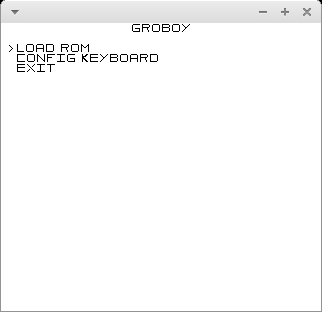
\includegraphics[scale=0.5]{images/screenshot_menu.png}
\caption{Capture du menu de la GUI}
\label{GUI1}
\end{figure}

\begin{figure}[!h]
\centering
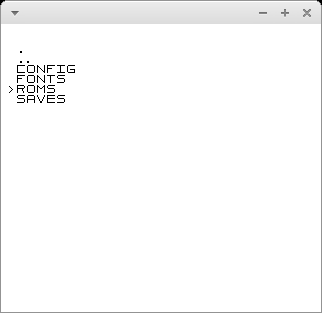
\includegraphics[scale=0.5]{images/screenshot_navigate.png}
\caption{Capture de la navigation dans les fichiers avec la GUI}
\label{GUI2}
\end{figure}

\begin{figure}[!h]
\centering
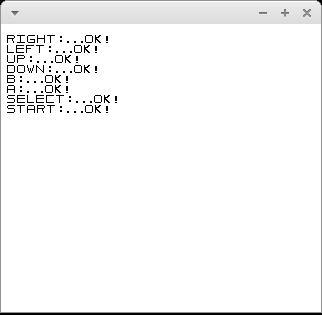
\includegraphics[scale=0.5]{images/screenshot_config.png}
\caption{Capture de la configuration des touches avec la GUI}
\label{GUI3}
\end{figure}

\begin{figure}[!h]
\centering
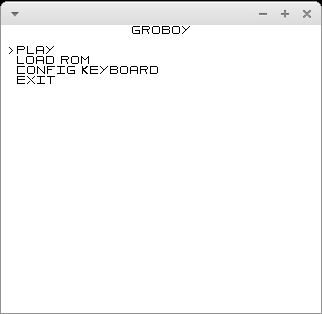
\includegraphics[scale=0.5]{images/screenshot_menu2.png}
\caption{Capture du menu après sélection d'un jeu avec la GUI}
\label{GUI4}
\end{figure}
\chapter*{Conclusion}
\section*{Bilan technique}
Au final, groboy est fonctionnel et jouable pour une grande majorité de jeux, nous allons lister pour chaque module le travail accompli. 
\subsection*{CPU}
Toutes les instructions sont bien implémentées, car groboy passe le test cpu de "blargg" sans erreur (cf. annexe C). 
\subsection*{GPU}
Le GPU travaille correctement, les trois couches de dessins sont bien implémentées, il est possible d'élargir l'écran comme le désire l'utilisateur.
\subsection*{APU}
Malgré une implémentation difficile à réaliser, le son est présent et tend à être fidèle au son d'origine.
\subsection*{Cartouches de jeu}
Les types de cartouche MBC1 et MBC2 ont été implémentés. Ce qui veut dire que l'ensemble des jeux utilisant ces puces sont jouables sur l'émulateur.
\subsection*{Sauvegarde}
Les sauvegardes classiques et par état sont implémentées.
\subsection*{GUI}
Une interface utilisateur est présente permettant de choisir un jeu, ou de reconfigurer les touches.
\section*{Fonctionnalités pouvant être rajoutées ou améliorées}
Dans cette partie nous allons parler des fonctionnalités principales qui peuvent être rajoutées ou améliorées.
\subsection*{Implémenter le comportement de cartouches MBC3}
Il manque pour que l'intégralité des jeux puissent être supportés d'implémenter les cartouches de types MBC3.
\subsection*{Améliorer le son}
Le son tend à être fidèle au son d'origine, cependant il ne l'est pas encore et rend par conséquent l'émulateur instable. Il faudrait pouvoir venir à bout de ce problème.
\subsection*{Implémenter le système deux joueurs}
La Game Boy dispose d'un port link pour pouvoir communiquer avec une autre Game Boy, il serait agréable de pouvoir faire de même entre deux processus groboy.
\subsection*{Implémenter la Game Boy Color}
La Game Boy Color a une architecture basée sur la Game Boy et donc très similaire, son portage est donc réalisable. 
\section*{Bilan collectif}
L'objectif principal de notre projet était l'étude d'un émulateur suffisamment abordable pour être réalisé, afin d'en tirer un maximum de connaissances sur le fonctionnement bas niveau d'un système relativement proche des ordinateurs que nous connaissons.
Si le physique de la machine et la personnalisation de son processeur par ses fabriquants laissent à penser qu'il n'y a aucun lien avec celles que nous utilisons, les idées que nous avons su tirer de ce projet nous ont, elles, donné un réel bagage pratique sur le fonctionnement de nos outils de travail préférés. 
De plus, le travail en équipe sur un projet relativement conséquent est toujours source d'apports utiles à nos futurs métiers. N'étant pas notre premier projet, les difficultés d'organisation furent moins nombreuses que les années précédentes, mais le développement de ce projet n'a pas été sans nous rappeler l'importance de bonnes prévisions, d'une bonne communication entre membres, et d'une répartition des tâches équitables.
Une fois de plus, le travail d'étude et de recherche est un véritable apport pour chacun de nous, tant sur l'aspect technique que sur l'expérience d'un travail sur un projet collectif, et peut-être même un premier pas dans le monde de l'émulation pour certains d'entre nous.
\section*{Emulation aujourd'hui}
Aujourd'hui l'émulation est un procédé extrêmement utile pour différentes tâches. Une des principales utilitées de l'émulation concerne les serveurs. Les serveurs actuels étant extrêment puissants, ils sont souvent utilisés dans les entreprises pour créer une multitude d'environnements de travail, en créant des machines virtuelles en leur sein. Cette technique est largement préconisée lorqu'il s'agit de gérer plusieurs logiciels sur un même serveur mais aussi pour créer des environnements de test. 
Les principales avancées et recherches actuelles dans le domaine de l'émulation concernent en grande partie, l'optimisation de la gestion des processus et la répartition des charges sur les différents coeurs pour les processeurs multi-coeurs.
%bibliographie
\bibliographystyle{plain}
\bibliography{rapport}
%annexes
\appendix
\chapter{Comptes rendus de réunion}
Durant notre projet, nous avons fréquemment été amenés à nous réunir, étudiants et encadrants, afin de discuter de l'avancée générale de notre travail.
Nombre de comptes rendus de ces réunions nous ont clairement guidé dans le développement.

Voici un exemple type d'un de ces comptes rendus, l'ensemble de ces derniers étant disponible via l'archive jointe au rapport.
\begin{quotation}
Compte rendu de la réunion de projet du 13/02/13\\
Travail réalisé :\\
	-Création des tables du Z80 (tables contenant tous les opcodes du processeur)\\
	-Ajout des fonctions de gestion du MBC1 et MBC2 (puces des cartouches Gameboy)\\
	-Une grande partie de la gestion de la mémoire a été implémentée\\
	-Rédaction et envoie de la feuille de route\\
	-Choix de trois articles en rapport avec notre sujet\\
Sujet abordé lors de la réunion :\\
	-Impossibilité de gérer les interruptions sans la partie graphique et sonore, de ce fait on ne peut tester correctement le processeur car celui-ci boucle sur certaines adresses mémoire car il attend une interruption et une modification de ces adresses\\
Objectifs pour la prochaine réunion :\\
	-Commencer la partie graphique et la partie son, pour pouvoir gérer les interruptions\\
	-Modifier le diagramme de Gantt (planning prévisionnel) pour qu’il reflète les changements de priorités dans les tâches\\
	-Faire un résumé des articles de recherche choisis en rapport avec notre sujet\\

Les deux diagrammes de Gantt celui créé après la première réunion et le nouveau sont joints au rapport.\\
\end{quotation}

\chapter{Blip buff et la génération d'ondes}
Le développeur "Blargg" cité en remerciements, a beaucoup travaillé sur les sons de synthèses à bandes passantes limitées, et principalement dans le cadre de l'émulation de systèmes de jeux relativement anciens, comme la Game Boy et la Nintendo NES par exemple. Ses travaux ont donc été d'une grande utilité pour le développement de la partie son de notre émulateur, sur laquelle la documentation est rare, avec notamment la librairie "blip buff" citée plus haut, qui permet de générer des ondes échantillonées à partir d'informations sur les ondes habituellement traitées par le processeur lui même. Par soucis d'efficacité et de temps, la programmation de ce module dépend fortemment du fonctionnement de cette librairie, c'est pourquoi nous avons choisi d'expliquer son fonctionnement général dans cette partie.\\
\section*{Vue d'ensemble}
Cette librairie réechantillonne donc des formes d'ondes audio à partir d'une fréquence d'horloge, vers une fréquence d'échantillonnage pour un signal.
Son utilisation suit généralement le schéma suivant :
- Créer un tampon mémoire avec la fonction 
\begin{lstlisting} 
		blip_new() 
\end{lstlisting}
- Paramétrer les fréquences d'horloge et d'échantillonage avec 
\begin{lstlisting} 
		blip_set_rates() 
\end{lstlisting}
- Lancer la boucle de génération d'onde :
\begin{itemize}
	\item Générer quelques basculement d'horloge avec 
	\begin{lstlisting}
			blip_add_delta()
	\end{lstlisting}
	\item Terminer le laps de temps avec 
	\begin{lstlisting}
			blip_end_frame()
	\end{lstlisting}
	\item Lire les échantillons dans le tampon avec 
	\begin{lstlisting}
			blip_read_samples()
	\end{lstlisting}
\end{itemize}
- Libérer le tampon avec 
\begin{lstlisting}
		blip_delete()
\end{lstlisting}

\subsection{Création du tampon mémoire}
Avant la création du son, un tampon mémoire doit être créé avec la fonction  "blip\_new()". Sa taille correspond au nombre maximum d'échantillons non lus qu'il contiendra. La plupart du temps, un dixième de la fréquence d'échantillonage suffit, puisque les échantillons seront généralement lus directement après leur génération.\\
La fonction "blip\_set\_rates()" permettra de fixer le nombre de pas d'horloge par seconde, et combien d'échantillons par seconde y correspondront. 
\subsection{Génération d'onde}
Par soucis de clarté, les exemples de cette section illustrent des ondes de faible amplitude, donc inaudibles. Des ondes codées sur 16 bits ont des valeurs allant de -32768 à + 32767.
Les ondes sont générées à la fréquence d'horloge en entrée.
Considérons une onde carrée simple avec 8 pas ("ticks d'horloge") d'horloge par cycle (4 pas hauts, 4 pas bas) : 

\begin{figure}[!h]
\centering
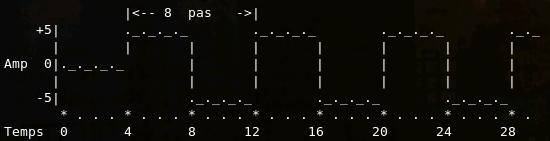
\includegraphics[scale=0.5]{images/Wave1.jpg}
\caption{Une onde carrée simple}
\label{WAV1}
\end{figure}

L'onde change d'amplitude aux points de temps 0, 4, 8, 12, 16, etc.
Le code suivant génère l'amplitude à chaque pas de l'onde ci-dessus à la fréquence d'horloge d'entrée : 
\begin{lstlisting}
int wave [30];
for(int i=4; i<30;++i){
	if( i%8 < 4)
		wave[i] = -5;
	else 
		wave[i] = +5;
}
\end{lstlisting}
Sans utiliser cette librairie, le tableau wave devrait ensuite être ré-échantillonné de la fréquence d'entrée à la fréquence d'échantillonnage de sortie. La librairie "blip\_buff" fait ce ré-échantillonage en interne, le code de génération de l'onde peut donc se focaliser entièrement sur l'horloge d'entrée.\\
Plutot que spécifier l'amplitude à chaque pas, blip buff n'a besoin que de connaître les points de basculement d'amplitude (i.e, où l'amplitude change, généralement à la demi période), qui sont nommés "deltas" par le développeur. Les temps correspondant à ces variations d'amplitudes sont donnés par des pas de l'horloge processeur (qui, dans notre cas, correspondent aux cycles du z80). 
Le schéma ci-dessous indique les "deltas" en dessous des points de temps auxquels ils interviennent.

\begin{figure}[!h]
\centering
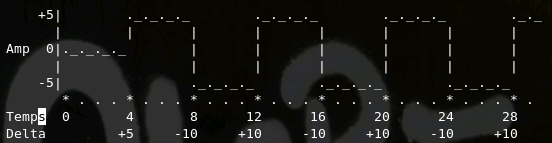
\includegraphics[scale=0.5]{images/Wave2.jpg}
\caption{L'intervention des deltas}
\label{WAV2}
\end{figure}

Le code suivant génère l'onde ci-dessus:
\begin{lstlisting}
blip_add_delta(blip, 4, +5);
blip_add_delta(blip, 8, -10);
blip_add_delta(blip, 12, 10);
blip_add_delta(blip, 16, -10);
blip_add_delta(blip, 20, 10);
blip_add_delta(blip, 24, -10);
blip_add_delta(blip, 28, 10);
\end{lstlisting}

\subsection{Gestion des laps de temps}
Le temps continuant d'augmenter, laisser l'onde avancer telle qu'elle provoquerait un dépassement de valeur d'entiers. 
La librairie permet d'éviter ceci en procédant à la génération de l'onde par laps de temps de longueur controlée.
Les pas d'horloge dans un laps de temps deviennent donc relatifs aux temps de début et de fin dudit laps.
Le temps de fin d'un laps de temps correspondra alors au temps de début du suivant.
Le schéma utilisé précédemment donne donc la division en laps de temps qui suit :

\begin{figure}[h]
\centering
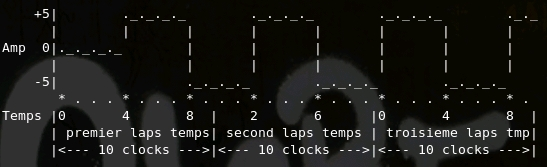
\includegraphics[scale=0.5]{images/Wave3.jpg}
\caption{Division en laps de temps}
\label{WAV3}
\end{figure}

Et cette onde peut etre générée par le code qui suit, dans lequel les échantillons sont sortis 10 par 10, et peuvent donc etre lus à la chaine sans risque de dépassement avec la fonction "blip\_read\_samples()".

\begin{lstlisting}
	blip_add_delta(blip,4,5);
	blip_add_delta(blip,8,-10);
	blip_end_frame(blip, 10);
	
	blip_add_delta(blip,2,10);
	blip_add_delta(blip,6,-10);
	blip_end_frame(blip, 10);
	
	blip_add_delta(blip,0,10);
	blip_add_delta(blip,4,-10);
	blip_add_delta(blip,8,10);
	blip_end_frame(blip, 10);
\end{lstlisting}

La longueur des laps de temps peut bien sur varier d'une lecture à l'autre.

Il existe une limite de 4000 échantillons de sortie par laps de temps, le nombre de pas d'horloge dépendant de la fréquence de cette dernière.
Pour des fréquences d'échantillonage classique, on arrive à des laps de temps d'un quinzieme de seconde, plus que suffisant pour nombre d'uilisations.

\chapter{Méthodes de débuggage et roms de test}
Le développement de la partie CPU a été épineux. Dans le sens où la moindre petite erreur immiscée dans le code pouvait mettre à mal l'ensemble de l'émulation. Fort heureusement il est trouvable sur internet des roms de domaine public accompagnées de leur sources permettant de tester le bon fonctionnement de l'émulateur. Ces roms ont été créées par un dénommé "Blargg" (le même individu qui a créé la librairie de son). Elles sont fiables car elles ont été testées avec une Game Boy physique. Dans ces roms il en existe une qui teste toutes les instructions du CPU, c'est elle que nous avons utilisé. Son principe est plutôt clair, la rom teste l'ensemble des instructions par groupe et vérifie pour chaque groupe si le résultat est correct grâce à un checksum. Si un groupe d'instructions échoue ce dernier est indiqué, sinon un message "ok" apparaît. Enfin il est possible de voir dans le code source quelles instructions ont eu un problème ce qui cible l'erreur immiscée dans le code de notre CPU. Grâce à ceci nous avons réussi à passer l'ensemble des instructions et par conséquent d'obtenir un CPU stable \ref{testcpu}.
\begin{figure}[!h]
\centering
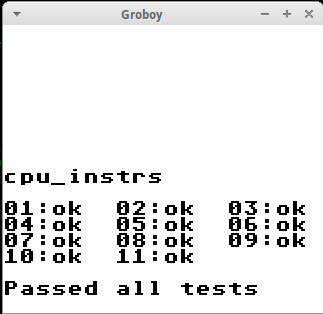
\includegraphics[scale=0.4]{images/screenshot_cpu_blargg.png}
\caption{Capture des tests réussis des instructions CPU avec groboy}
\label{testcpu}
\end{figure}
\end{document}
